%--------------------
% Packages
% -------------------
\documentclass[preprint,12pt, authoryear]{elsarticle}
\usepackage[T1]{fontenc}
\usepackage[utf8x]{inputenc}
%\usepackage{gentium}
\usepackage{mathptmx} % Use Times Font
\usepackage{amsfonts} %for math notation

\usepackage[pdftex,linkcolor=black,pdfborder={0 0 0}]{hyperref} % Format links for pdf
\usepackage{graphicx}
\usepackage{calc} % To reset the counter in the document after the title page
\usepackage{enumitem} % Includes lists
\usepackage{natbib}
\usepackage{verbatim}
\usepackage{subcaption}

\frenchspacing % No double spacing between sentences
\linespread{1.2} % Set linespace
\usepackage[a4paper, lmargin=0.1666\paperwidth, rmargin=0.1666\paperwidth, tmargin=0.1111\paperheight, bmargin=0.1111\paperheight]{geometry} %margins
%\usepackage{parskip}

\usepackage[all]{nowidow} % Tries to remove widows
\usepackage[protrusion=true,expansion=true]{microtype} % Improves typography, load after fontpackage is selected

\usepackage[version=4]{mhchem} % Formats chemical forumla

\usepackage{lipsum} % Used for inserting dummy 'Lorem ipsum' text into the template

\usepackage{booktabs, multirow} % for borders and merged ranges
\usepackage{soul}% for underlines
\usepackage[table]{xcolor} % for cell colors
\usepackage{changepage,threeparttable} % for wide tables
\usepackage{colortbl,xcolor}
\usepackage{rotating} % Required for sidewaystable
\definecolor{customgreen}{HTML}{74B652}
\definecolor{custompurple}{HTML}{7B52AE}

\usepackage{appendix} % To use the appendix environment
\usepackage{url}
\usepackage{boxedminipage}
\usepackage{textpos}
%-----------------------
% Begin document
%-----------------------
\journal{Transportation Research Part A}

\begin{document}
\begin{frontmatter}

\title{Examining the causal impacts of the built environment on cycling activities using time-series street view imagery}

% Author details
\author[doa]{Koichi Ito}
\author[dcee]{Prateek Bansal}
\author[doa,dre]{Filip Biljecki\corref{cor1}}

\affiliation[doa]{organization={National University of Singapore, Department of Architecture},%Department and Organization
            addressline={8 Architecture Drive}, 
            city={Singapore},
            postcode={117356}, 
            country={Singapore}}
\affiliation[dcee]{organization={National University of Singapore, Department of Civil and Environmental Engineering},
            addressline={1 Engineering Drive}, 
            city={Singapore},
            postcode={117576}, 
            country={Singapore}}
\affiliation[dre]{organization={National University of Singapore, Department of Real Estate},%Department and Organization
            addressline={15 Kent Ridge Drive}, 
            city={Singapore},
            postcode={119245}, 
            country={Singapore}}

\cortext[cor1]{Corresponding author. Email: filip@nus.edu.sg}



\begin{abstract}
\begin{textblock*}{\textwidth}(0cm,-11.5cm)
\begin{center}
\begin{footnotesize}
% \vspace*{-13cm}
\begin{boxedminipage}{1\textwidth}
This is the Accepted Manuscript version of an article published by Elsevier in the journal \emph{Transportation Research Part A} in 2024, which is available at:\\ \url{https://doi.org/10.1016/j.tra.2024.104286}\\ Cite as:
Ito K, Bansal P, Biljecki F (2024): Examining the causal impacts of the built environment on cycling activities using time-series street view imagery. \textit{Transportation Research Part A: Policy and Practice}, 190: 104286.
\end{boxedminipage}
\end{footnotesize}
\end{center}
\end{textblock*}

\begin{textblock*}{1.5\textwidth}(-0.8cm,17.3cm)
{\tiny{\copyright{ }2024, Elsevier. Licensed under the Creative Commons Attribution-NonCommercial-NoDerivatives 4.0 International (\url{http://creativecommons.org/licenses/by-nc-nd/4.0/})}}
\end{textblock*}
Cycling is vital for sustainable and healthy cities. To encourage such activities, understanding urban bikeability at both detailed and broad spatial scales is crucial. Street view imagery (SVI) offers in-depth insights into how street features influence micro-mobility patterns, but existing studies are mainly correlational. This research utilized historical time-series SVI, cyclist data from London, to discern the causal effects of specific urban features on cyclist numbers. We used propensity score matching to adjust for potential confounding biases and applied the causal forest to estimate the heterogeneity in causal effects. Key findings include: vegetation significantly boosts cycling, slope negatively impacts cycling, and bike lanes positively influence cycling. Moreover, vegetation's impact on cycling is greater in less populated areas, while bike lanes have a stronger effect in densely populated regions. These findings help prioritize the areas of intervention. By transcending from mere correlations to identifying heterogeneous causal impacts, this study offers invaluable insights for urban planning, underscoring design strategies to enhance cities' bikeability and sustainability.
\end{abstract}

% %%Graphical abstract
% \begin{graphicalabstract}
% 	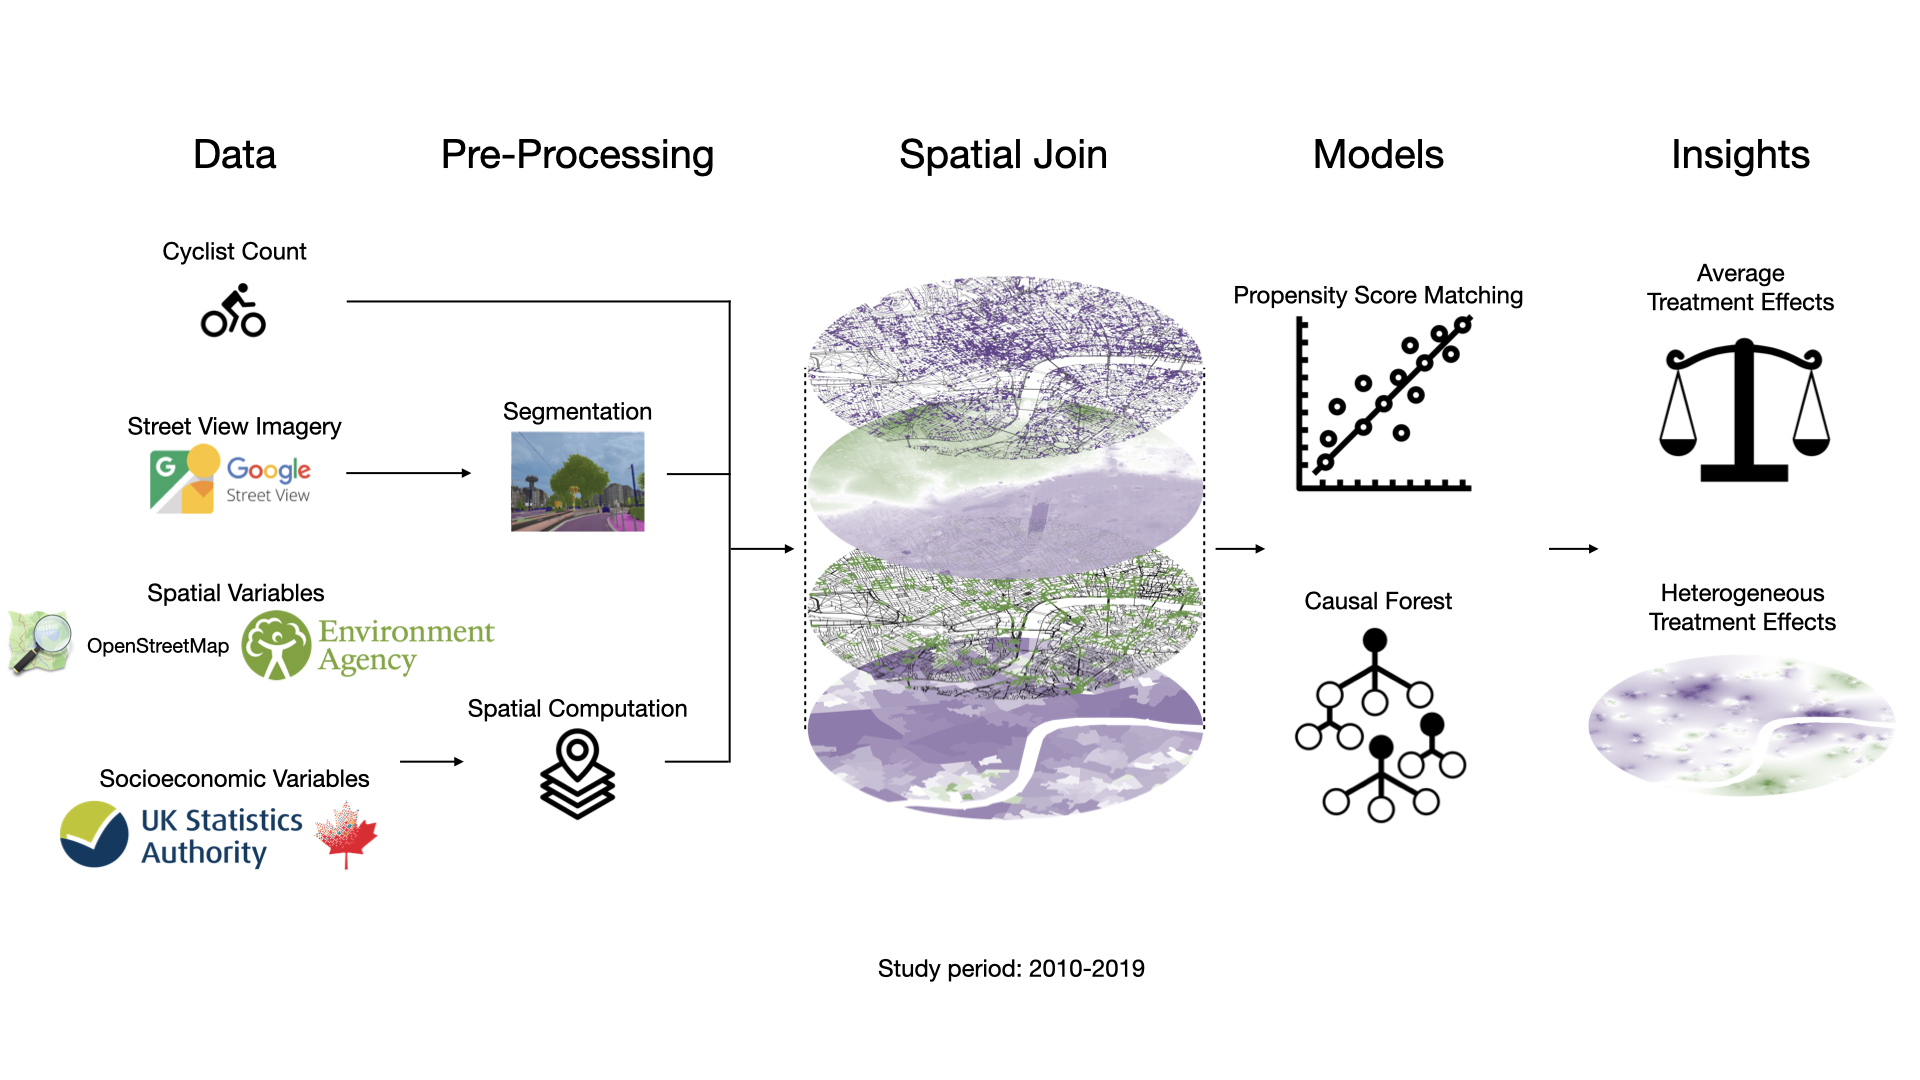
\includegraphics[width=\textwidth]{fig/workflow.003.png}
% \end{graphicalabstract}

% %%Research highlights
% \begin{highlights}
% \item Examined causal relationships between street features and cycling mobility.
% \item Utilized historical SVI data and cyclist count data in London.
% \item Revealed the effects of urban design on cycling activities.
% \item Identified heterogeneous treatment effects of urban design interventions.
% \end{highlights} 

\begin{keyword}
Urban design \sep Active transportation \sep Propensity score matching \sep Causal forest \sep Deep learning
\end{keyword}

\end{frontmatter}

\section{Introduction} \label{sc:intro}
Promoting active transportation (i.e.\ walking and cycling) is critical to make urban transportation green and healthy \citep{neves_assessing_2019, cao_contribution_2019}. To understand the factors promoting cycling, researchers have developed and analyzed bikeability indexes (i.e., indexes that represent cyclist-friendliness), including examining the impact of specific sub-indicators such as greenery and sky view factor on cycling activities \citep{biljecki_street_2021a, fry_assessing_2020, mahabir_crowdsourcing_2020,2023_epb_semantic_networks}. Recent studies have utilized street view imagery (SVI) data to explore these relationships, leveraging the high-quality and extensive availability of SVI to identify correlations between street features and active transportation usage to validate whether sub-indicators contribute to active mobility usage \citep{yang_global_2020, nagata_objective_2020, wang_relationship_2020}. However, studies on the urban scale may encounter confounding biases due to the observational nature of the data. Neighborhood characteristics such as population and employment densities can influence both the implementation of urban design elements (e.g., slope, vegetation, separate bike lanes) and the extent of cycling activities.
For example, \autoref{intro:fig:propensity} shows a probability of having vegetation in London, illustrating how such a characteristic is not evenly distributed throughout the city. If areas with lower population densities are more likely to receive more vegetation, this distribution could reflect underlying preferences or needs rather than a random assignment of urban greenery. This scenario underscores the concept of selection bias, where the observed effect of more vegetation on promoting cycling might be confounded by the inherently higher cycling rates in densely populated areas.

Moreover, historical SVI data have not been utilized to match with existing time-series cyclist count data, only using the latest data and discarding many historical data points. Therefore, existing studies are statistically limited and may not provide reliable results.

This study aims to bridge such research gaps by examining the causal effect of various urban design elements on cyclist count by leveraging large-scale time-series SVI data in combination with state-of-the-art causal inference techniques. To address the potential confounding biases, we adopted propensity score matching (PSM) with bike lanes, street parking, street lights, vegetation, and slope as treatments for cycling activity. We subsequently took advantage of recent advancements in tree-based causal inference methods to analyze heterogeneous treatment effects, which enable policymakers to gain more nuanced insights into what contributes to bikeability and what drives differing treatment effects \citep{athey_generalized_2019}.

This research is the first to investigate the causal relationships between the built environment and active transportation at an urban scale and examine the heterogeneous treatment effects, thereby providing valuable insights into the effects of urban design for urban planners and policymakers and contributing to more transparent cycling infrastructure investment \citep{meng_political_2022}. The paper is structured as follows. Section \ref{sc:lit_review} reviews the literature on the application of SVI in the micromobility domain. Section \ref{sc:data_method} presents the data extraction process and key fundamentals of the adopted causal inference approaches. The results and their implications for policymakers are detailed in Section \ref{sc:result}. The final section, Section \ref{sc:conclusion}, concludes with the main takeaways and highlights limitations and avenues for future research.

\begin{figure}
    \centering
    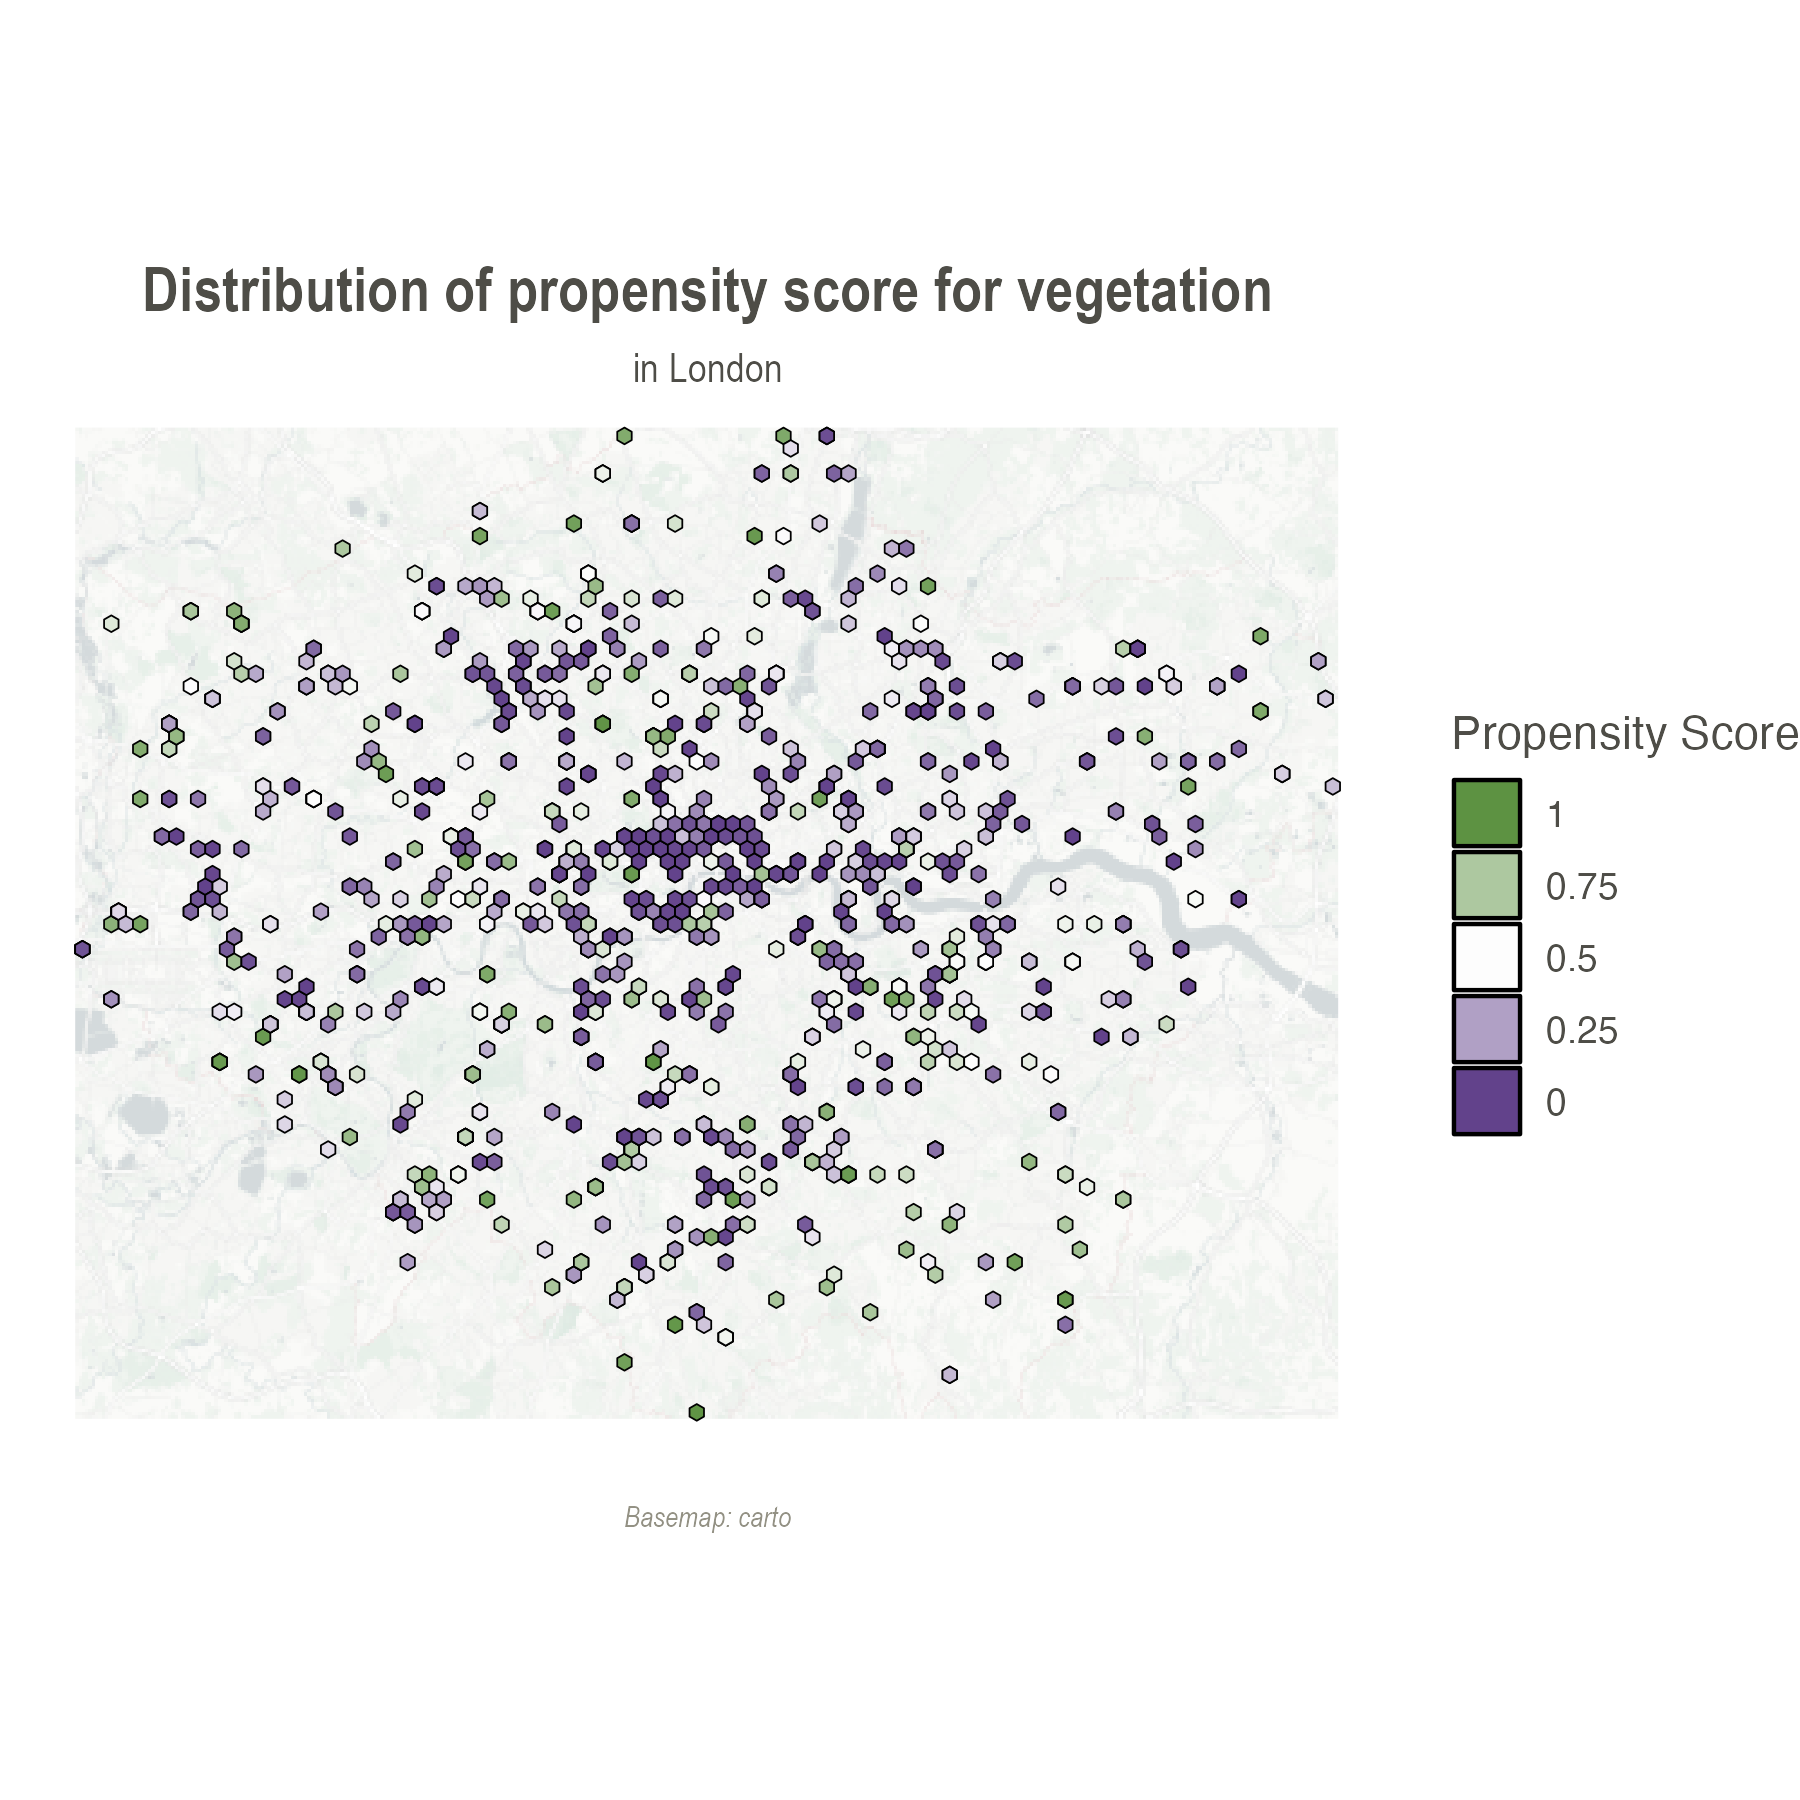
\includegraphics[width=\textwidth]{fig/London/vegetation/ss_vegetation_binary_propensity_score_map.png}
    \caption{A map of propensity score of having wider vegetation (i.e., above 70 percentile of all observations). Spatial heterogeneity can be observed, indicating potentially non-random assignment of treatment (i.e., more vegetation).}
    \label{intro:fig:propensity}
\end{figure}


\section{Literature review}  \label{sc:lit_review}
The importance of transportation has motivated a multitude of studies to assess bikeability in cities, which have often been conducted by taking a weighted average of a set of indicators that are considered to contribute to the cyclist-friendliness of streets and areas \citep{frank_development_2010, ewing_measuring_2009, duncan_validation_2011, wysling_where_2022, hosford_15minute_2022, codina_built_2022, bao_understanding_2023}. 
Previous studies used neighborhood-level indicators, such as land use mix and population density, subjective indicators, such as the qualitatively estimated proportion of sky seen from cyclist perspectives, and topographical characteristics. 

Many researchers have taken advantage of the expanding coverage of SVI and the scalable data collection process to understand the perceptions of cyclists and develop these indexes on an urban scale \citep{ito_understanding_2024, yin_measuring_2016, li_investigating_2018}. Some studies manually audited these images to conduct a systematic assessment using a predefined checklist \citep{yin_street_2017, gu_using_2018, yoo_are_2024}. Recent developments in computer vision techniques have enabled recent studies to quantify a few sub-indicators that are often included in active mobility indexes, such as greenery and sky view fact, bike lane, and subjective perception scores (e.g., safety) \citep{wang_relationship_2019, wu_does_2020, basu_how_2022, zeng_measuring_2024}. Subsequently, a handful of studies have constructed comprehensive bikeability indexes based on information extracted from SVI with CV by incorporating not only infrastructure-related indicators, such as bike lanes and traffic lights but also perception-related indicators, such as safety and beauty of streets \citep{wang_linkage_2019, ito_assessing_2021a, koo_development_2022}. 

It has also been increasingly popular to examine correlations or build predictive models with cycling-related variables (e.g., count data, accident data, and trajectory data) and sub-indicators of bikeability from SVI \citep{yang_global_2020, nagata_objective_2020, wang_relationship_2020, hankey_predicting_2021, zhou_assessing_2023, ye_unpacking_2024, rui_built_2024, xue_integrating_2024, zhao_preferred_2024, gong_deciphering_2024, wang_evaluating_2024, vega_assessing_2024}.
Moreover, very few studies have used historical SVI data to analyze urban environments despite its usefulness in matching with other historical data and ensuring more data points \citep{liang_revealing_2023, stalder_selfsupervised_2024}.
On the one hand, the factors and policy interventions (e.g., infrastructure and educational programs) that can affect cycling patterns have also been researched extensively with causal inference methods \citep{burbidge_evaluating_2009, aittasalo_socioecological_2019, hong_can_2020, li_effects_2019, kearns_increasing_2019, vidaltortosa_cycling_2021, piras_could_2021}.
On the other hand, despite the increasing number of correlational papers, almost no study has been conducted to infer causality of these sub-indicators and interventions.

In summary, previous studies have used SVI to derive indexes or correlations between elements of urban design and the extent of active transportation. None of these studies has considered potential confounding biases. On the other hand, there is a rich literature on estimating the causal effect of infrastructural interventions on cycling activities. However, no studies have taken advantage of the street characteristics recovered from the widely available large-scale SVI data \citep{molenberg_systematic_2019}. This study addresses this research gap and advances the application of SVI in obtaining more concrete policy-relevant implications by addressing potential confounding biases through state-of-the-art causal inference approaches. 
Through the literature review, we identified relevant sub-indicators of bikeability that are mainly extractable from SVI and decided to use them as treatment variables because they can be modified through interventions (see \autoref{lit_review:tab:treatment}).
We also found that previous studies have reported the influence of the following variables on people's travel patterns: housing price, income levels, age groups, land use, point-of-interest (POI) and population density \citep{anas_discrete_1984, vasudevan_determining_2021, odriscoll_how_2023, zhang_role_2004, king_does_2015, frank_impacts_1994}. 
Thus, we included them in the subsequent analyses.

\begin{table}[!htp]\centering
\caption{This table shows a list of indicators of bikeability used in previous studies with their identified effect directions and study areas. We decided to use them as treatment variables because they can be modified through interventions.}\label{lit_review:tab:treatment}
\tiny
\begin{tabular}{lrrr}\toprule
\textbf{Variables} & \textbf{Studies that found them positive} & \textbf{Studies that found them negative} & \textbf{Studies that found them inconclusive} \\\midrule
Vegetation & \begin{tabular}[r]{@{}r@{}}\citet{yang_global_2020} in Hong Kong,\\ \citet{nagata_objective_2020} in Tokyo,\\ \citet{wang_relationship_2020} in Shenzhen\end{tabular} & - & -\\
Bike Lane & \begin{tabular}[r]{@{}r@{}}\citet{parker_installation_2011} in New Orleans,\\ \citet{goodno_evaluation_2013} in Washington, D.C.\end{tabular} & - & -\\
Street Parking & - & \begin{tabular}[r]{@{}r@{}}\citet{torrance_effects_2009} in Texas,\\ \citet{ito_assessing_2021a} in Singapore and Tokyo\end{tabular} & -\\
Street Light & \begin{tabular}[r]{@{}r@{}} \citet{uttley_road_2020} in Birmingham, \\ \citet{chen_gps_2018} in Seatle \end{tabular}& - & - \\
Slope & - & \citet{broach_where_2012} in Portland & \citet{wahlgren_exploring_2014} in Stockholm \\\bottomrule
\end{tabular}
\end{table}

\section{Data and Methods} \label{sc:data_method}
The overall workflow of this study is shown in \autoref{methodology:fig:workflow}. For study areas, we chose London for its comprehensive lists of publicly available data, most of which are yearly updated and suitable for our time-series analysis with many control variables. The dependent variable in this study is the cyclist count data from London. Features such as bike lanes, street parking, street lights, and vegetation were automatically extracted from SVI, and the slope was obtained from spatial data (i.e., digital terrain model). After computing visual features, spatial variables, and socioeconomic indicators, PSM and causal forest were adopted to infer causal effects of various indicators, namely, bike lanes, street parking, street lights, vegetation, and slope as treatments for cycling activity. Treatment indicators and their nature were selected based on the literature review (see \autoref{lit_review:tab:treatment}) so that policymakers, urban planners, and urban designers can amend them.

In our study, we used both PSM and causal forest models to leverage their complementary strengths in causal inference.
PSM is used to mitigate confounding by matching similar treated and untreated units, effectively simulating the conditions of a randomized trial for bias reduction.
Causal forests, on the other hand, excel in identifying how treatment effects vary between different subgroups by modeling complex interactions within the data. This integrated approach ensures the robustness of our findings, allowing for a detailed examination of both the average and heterogeneous effects of urban design on cyclist count.

By utilizing both methods, we achieve a balance between controlling for confounding variables and uncovering nuanced effect variations, enriching our analysis with a comprehensive perspective on causal relationships.
This study uses aggregated level analysis to focus on the total counts of cyclists, effectively summarizing the collective outcome of individual decision-making processes. This approach is chosen for its ability to estimate the effects of treatment variables on the aggregate number of cyclists at specific locations. Aggregated level data is appropriate for our objectives, as it allows for the examination of how urban design interventions influence overall patterns of active transportation \citep{molenberg_systematic_2019, xiao_impacts_2022, xiao_design_2023, tait_build_2024}. This methodology enables policymakers, urban planners, and urban designers to understand the broader implications of their decisions on active transportation trends, providing a solid foundation for informed urban development and policy formulation.

\begin{figure}
    \centering
    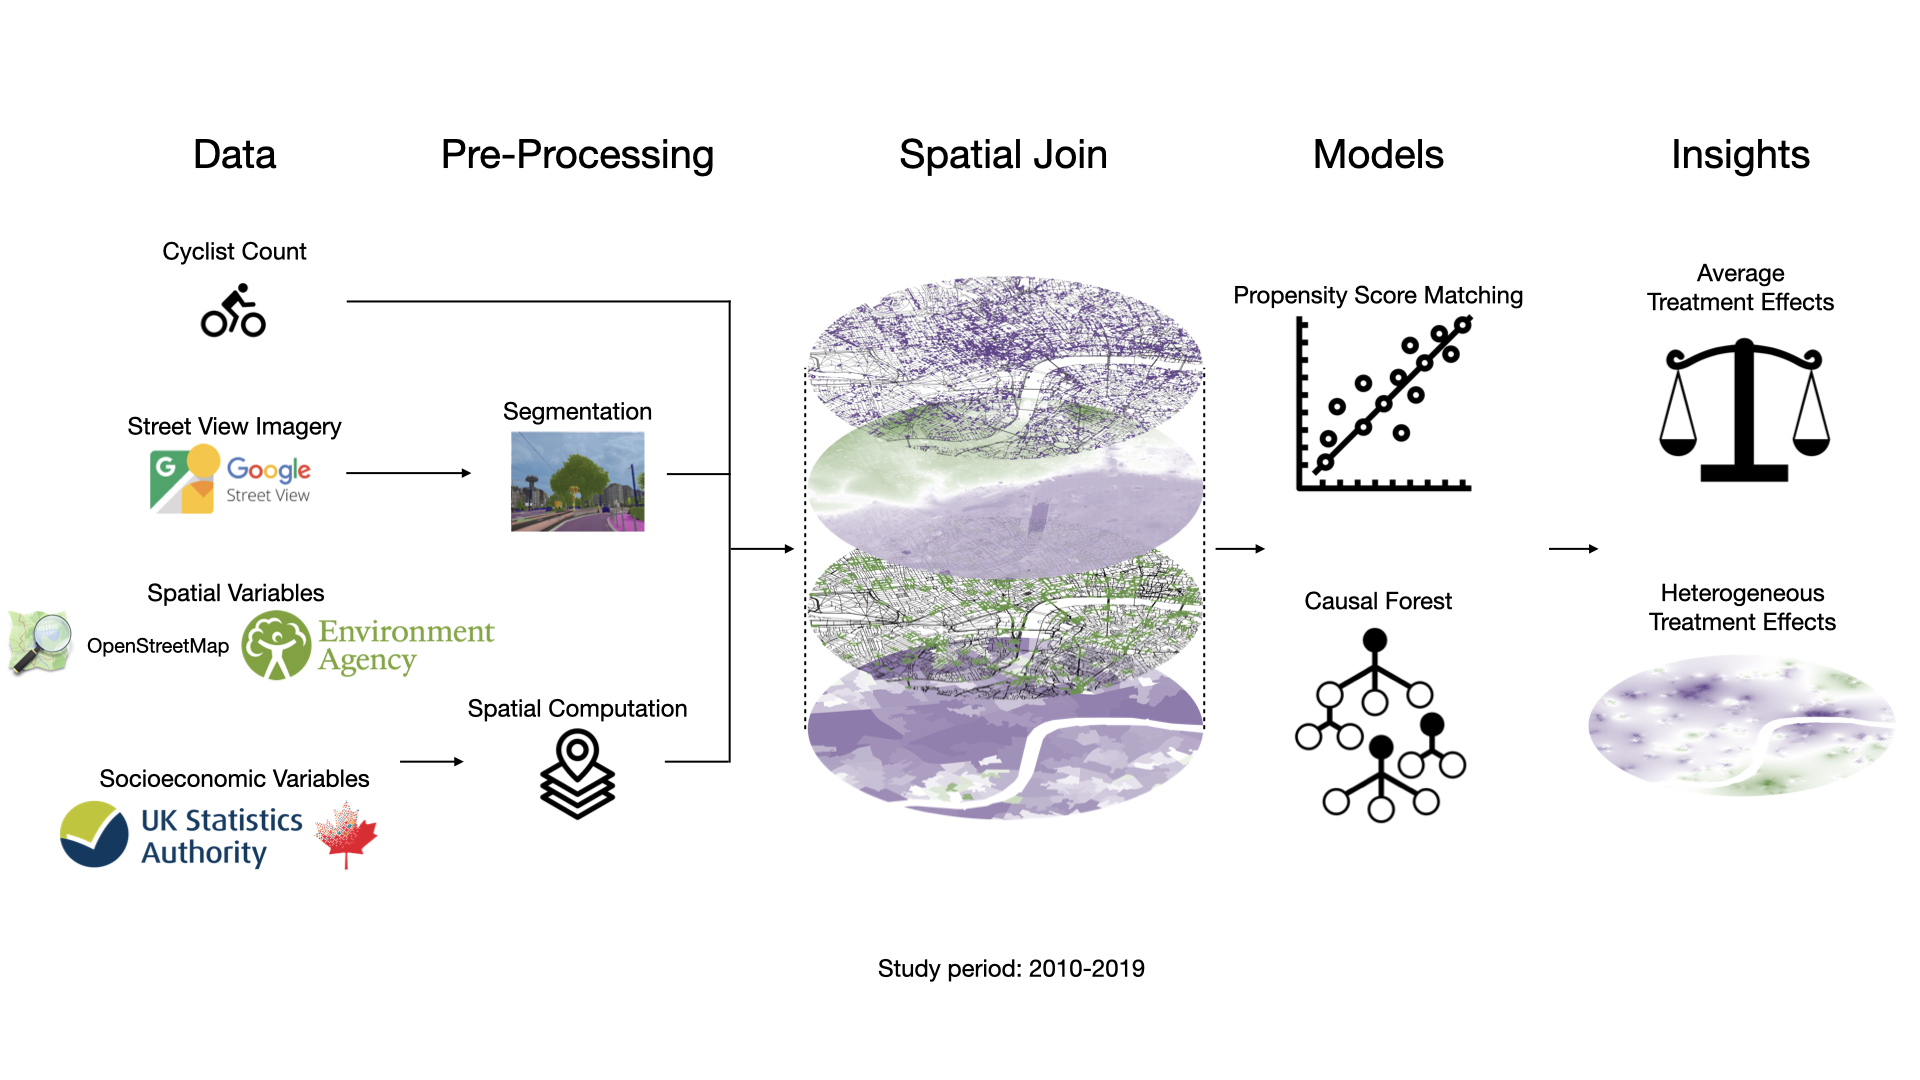
\includegraphics[width=\textwidth]{fig/workflow.003.png}
    \caption{Overall workflow of this study.}
    \label{methodology:fig:workflow}
\end{figure}

\subsection{Data}
To quantify cycling activities, this study used cyclist count data collected by the Department of Transport in London \citep{DfT2022}. This dataset contains cyclist counts at more than 3,000 fixed count points in the Greater London area, which have been collected once a year since 2000. This study calculated the average daily total count during the day from 07:00 to 19:00 at each count point for the available months between 2010 and 2019, and each count was used as the unit of analysis for this study.

To provide a more contextualized overview, we visualized the changes in the count data between 2010-2014 and 2015-2019 in London in \autoref{data:fig:count_maps}, where the increases in the count are shown in green and decreases in purple. Increases in the count were observed in central areas of London, and the photos on the left side of the plots show the changes in the built environment over time in London (e.g., the addition of separated bike lanes).
\autoref{data:fig:count_ridge} shows changes in the distribution of cyclist counts in London.
London saw a slight increase in the density of count over 250 over the years.

\begin{figure}
    \centering
    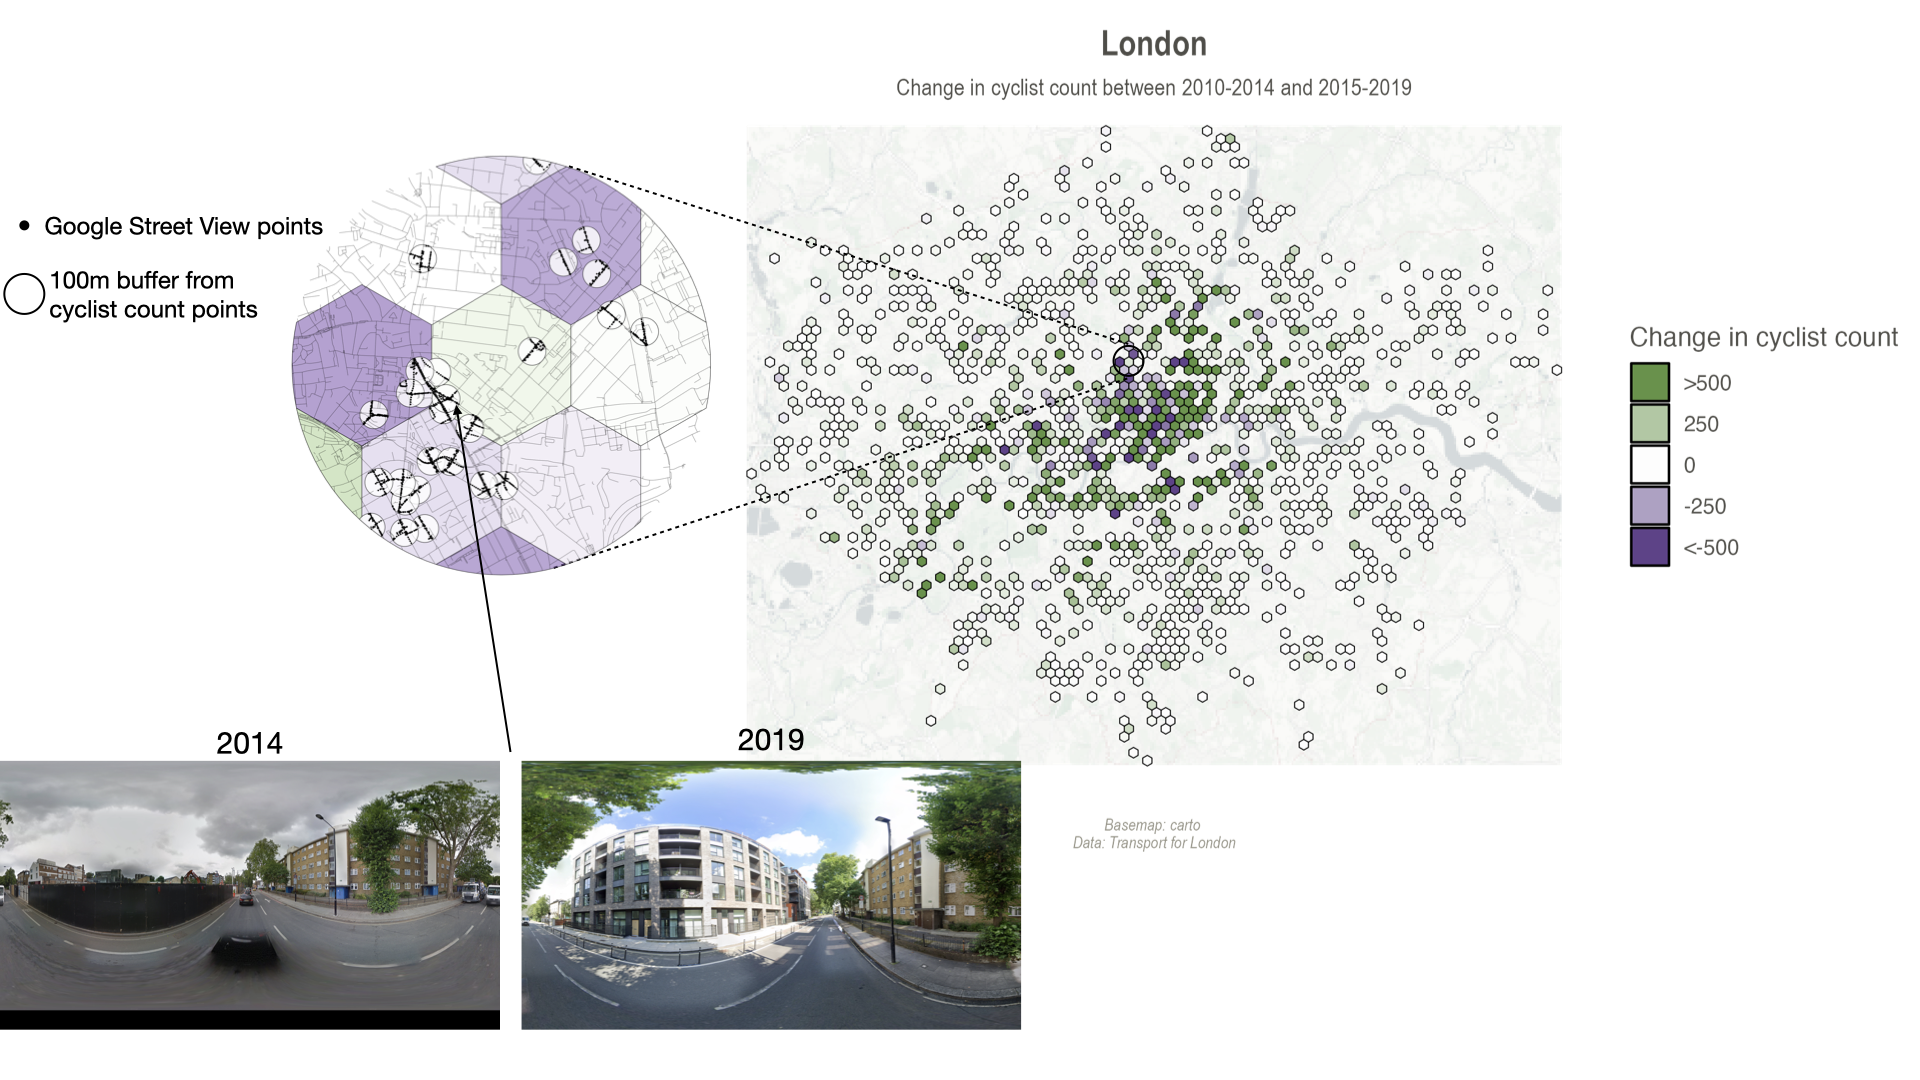
\includegraphics[width=\textwidth]{fig/London/workflow.006.png}
    \caption{This map shows the changes in the number of cyclists over time in parts of London. The cells represent aggregated locations of count stations. The greener color indicates an increase in the count, and the purpler color indicates a decrease. The zoomed-in views on the left side of the map show 100m buffers around count stations and SVI points within them. In the bottom left corner, the photos display examples of SVI in 2010-2014 and 2015-2019 in London to show the changes in the built environment. Source of the imagery: Google Street View. Source of the base map: carto.}
    \label{data:fig:count_maps}
\end{figure}

\begin{figure}
    \centering
    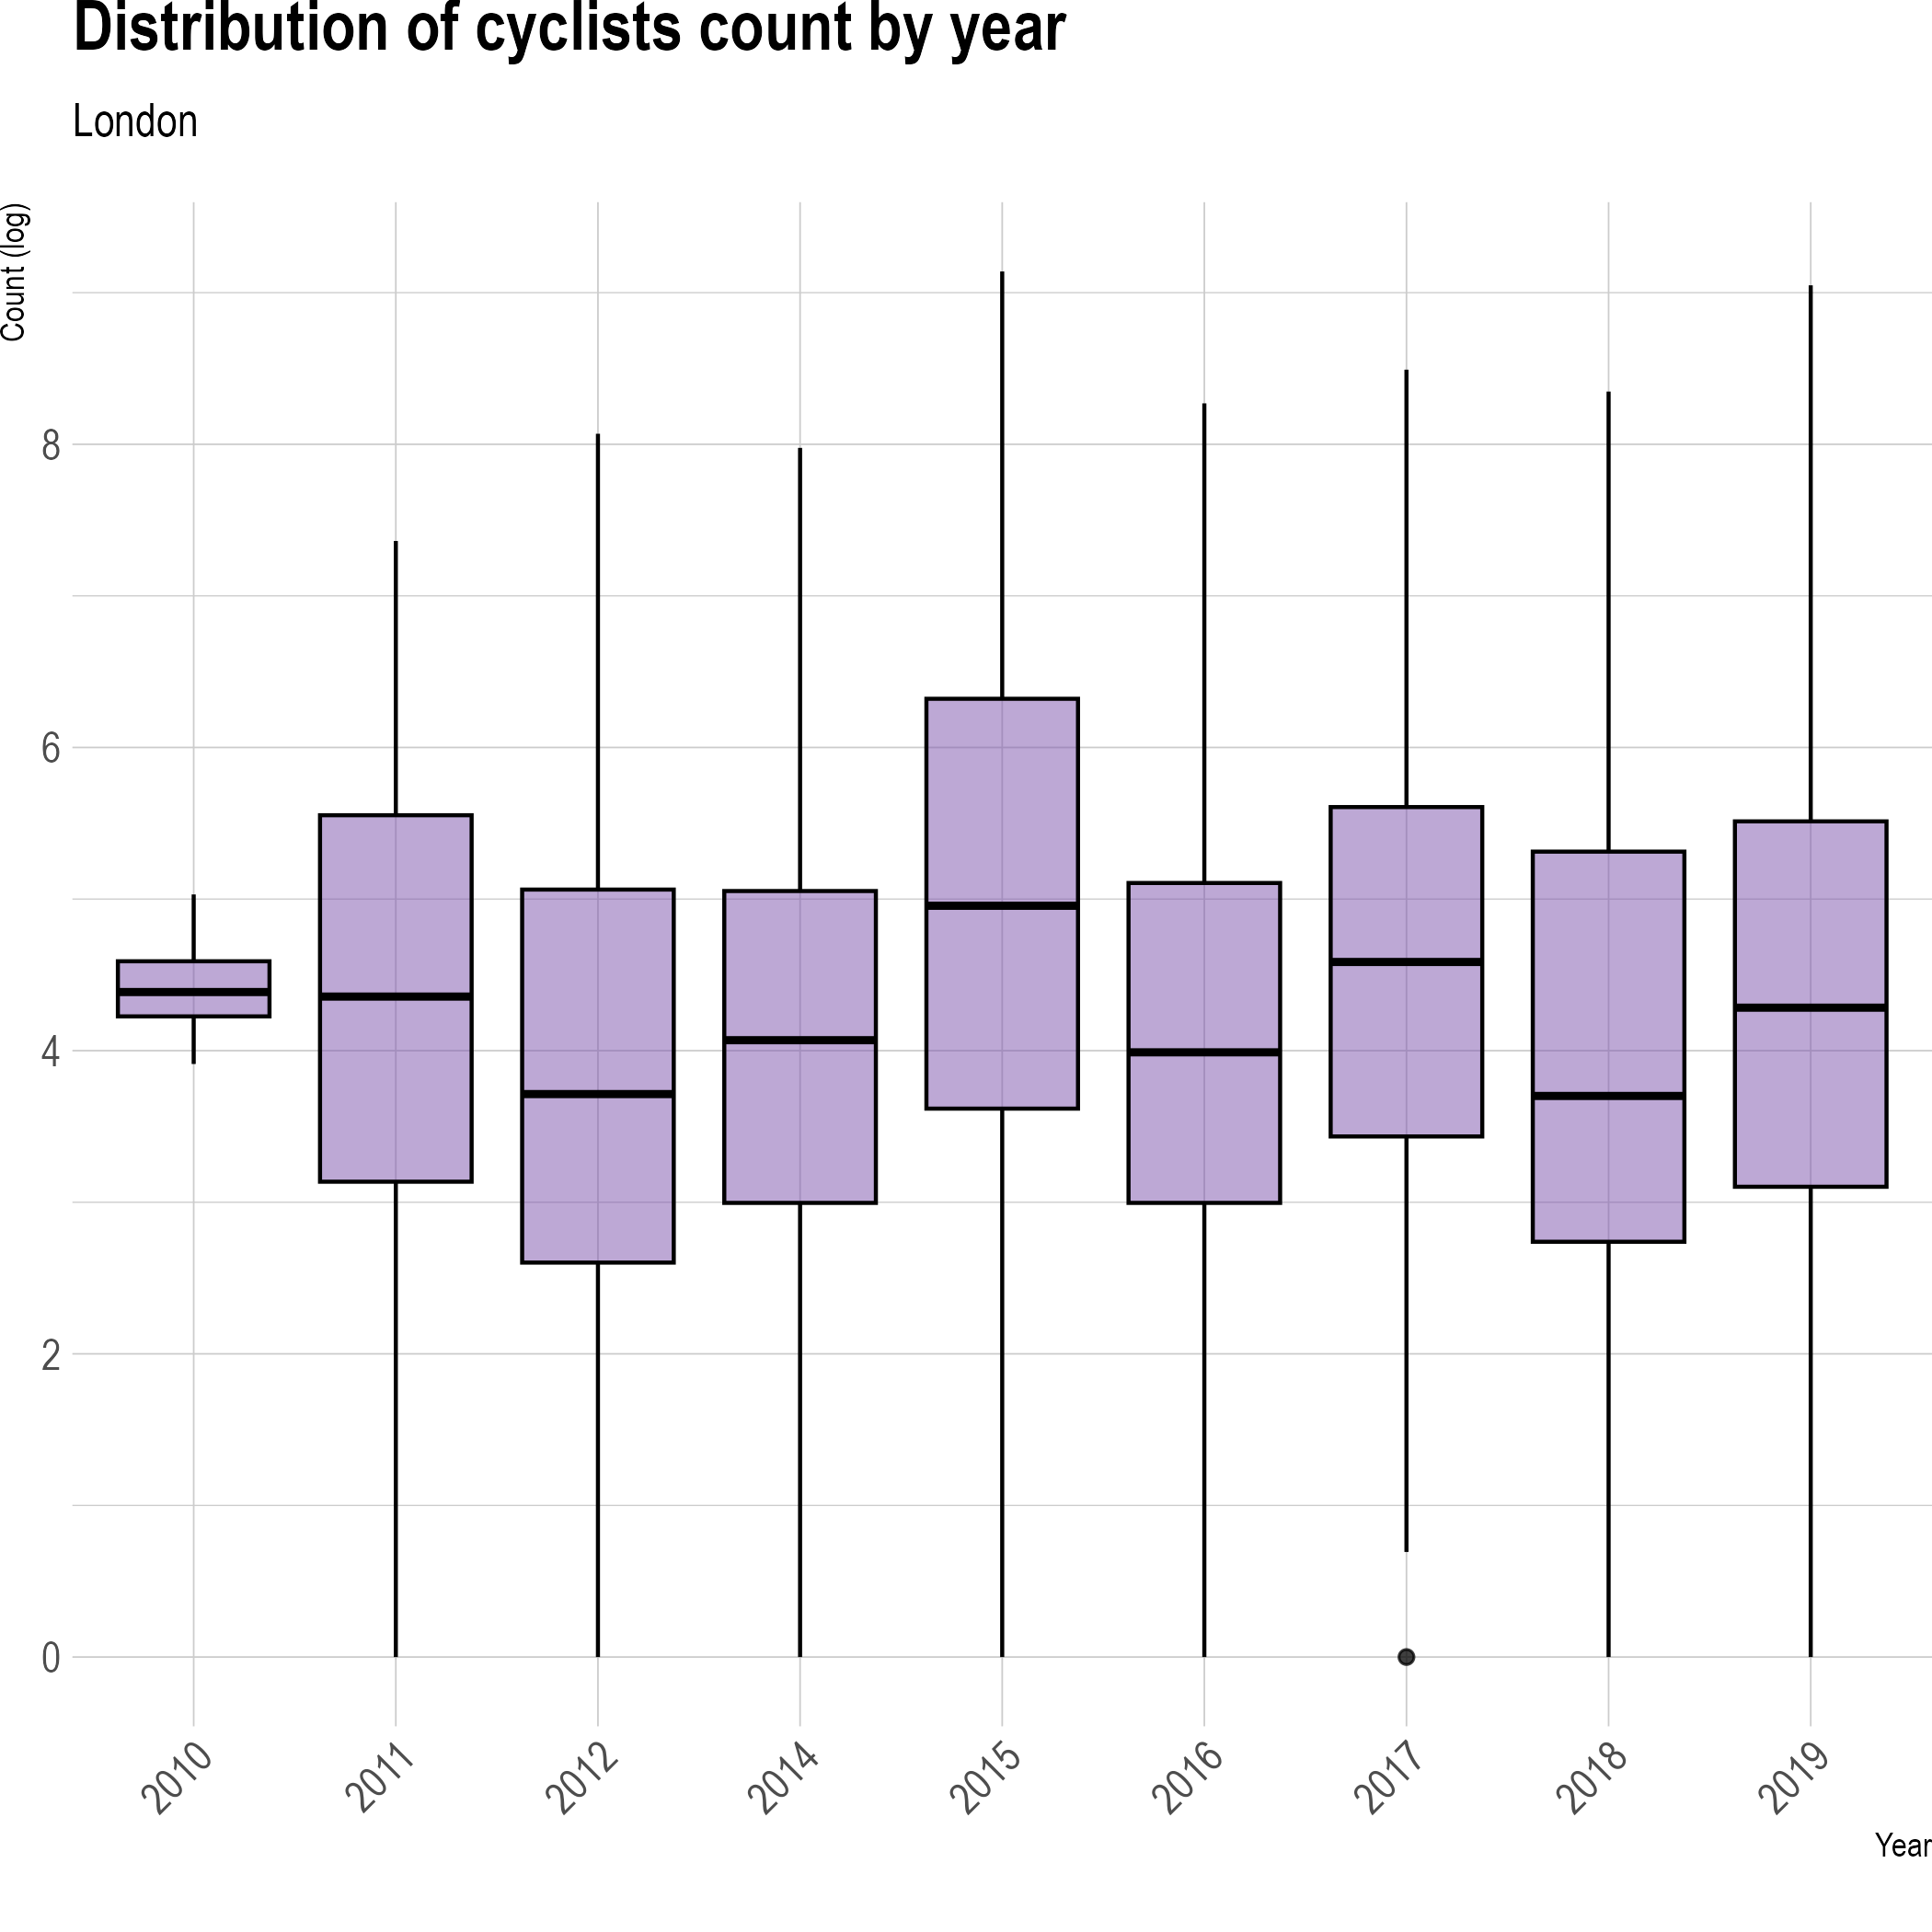
\includegraphics[width=0.6\textwidth]{fig/London/count_boxplot.png}
    \caption{This box plot shows the distribution of cyclist counts (log) in London by year.}
    \label{data:fig:count_ridge}
\end{figure}

All the independent variables used in this study are available for each year, making it panel data. Average daily counts are available for each month over the years, enabling us to use year- and month-specific fixed effects to control for monthly and yearly variation in unobserved factors such as weather. As for the SVI data, this study collected historical data from Google Street View between 2010 and 2019 using the location of the count points \citep{google_google_2023}. This study also collected conventional spatial data that bikeability studies have often used \citep{ito_assessing_2021a,winters_bike_2016}, namely the slope of the terrain and points of interest (POIs), such as shops and health care facilities. For terrain data, we used LiDAR data at a 10-meter resolution collected by the UK government in 2019, while for POI data, we utilized OpenStreetMap historical data since 2007 provided by \citep{raifer_oshdb_2021}.

To control for other socioeconomic variables, this study included the following variables: demographic data, deprivation data, housing price, and land use data. Demographic data for each Lower-Layer Super Output Area (LSOA) in the Greater London area is provided by the Office for National Statistics in the UK \citep{londondatastore_indices_2023}. Based on their data, age composition grouped by 10 years was computed from the raw data (i.e.\ population from 0 to 9 years old as a group), and the population density per $km^2$ was calculated.
To account for the comprehensive socioeconomic status of the neighborhood, this study used the Index of Multiple Deprivation (IMD) provided by the UK Ministry of Housing, Communities, and Local Government.
As for housing prices and land uses, data provided by the Land Registry and Department for Levelling Up, Housing and Communities were used for London.

The selection of variables for this study was guided by the objective of capturing the multifaceted influences on cycling. Land use and POIs were included as proxies for activity generators that attract people to visit. To account for accessibility to these origins and destinations, we also included street network-related variables such as the number of times the street segment was used as the shortest route between major origins and destinations and accessibility to POIs. Additionally, to control for the safety of cyclists, the traffic speed limit from OpenStreetMap was used as a proxy for the actual traffic speed on the street. We also did not include another potential variable that could affect cyclists, a perception of safety, because a previous study has reported that its variance can be explained by the results of the semantic segmentation alone \citep{beaucamp_whole_2022}.  

\subsection{Methods}
\subsubsection{Variable construction}
To quantify the visual features of the streets of SVI, image semantic segmentation was carried out. 
We selected a state-of-the-art computer vision model called Mask2Former pre-trained on the Mapillary Vistas dataset with 65 categories and 64.7\% Mean Intersection over Union (mIoU --- the average ratio between the intersection and the union of the predicted and ground truth segmentation areas across all classes), and this model has increasingly been used by many urban science studies \citep{cheng_maskedattention_2022, yap_urbanity_2023, li_evaluation_2023, yap_global_2023}.
Based on the result of segmentation, we also computed visual complexity, which is entropy to reflect the diversity of visual features in SVI~\citep{2023_epb_semantic_networks} (see \autoref{methodology:equation:vis_complexity}).

\begin{equation}
VC =-1\left(\sum_{i=1}^{n} p_{i} * \ln (p_{i})\right) / \ln (n)
\label{methodology:equation:vis_complexity}
\end{equation}

In this equation, $VC$ is the visual complexity, $pi$ denotes the pixel ratio of category $i$, and $n$ represents the total number of categories. A visual complexity score of 1 means the most diverse mix of visual features possible, while a score of 0 indicates that SVI has only one category. Adding this indicator to the set of distinct categories can capture the overall complexity of visual input that street users experience on particular streets. In addition to semantic segmentation, panoptic segmentation was performed with the segmentation model mentioned above to quantify the share of transport modes inferred from SVI by counting the number of vehicles, bicycles, and pedestrians \citep{carion_endtoend_2020, lin_microsoft_2015}. 
\autoref{method:fig:segmentation_example} showcases the results of panoptic segmentation (that is, a model that combines semantic segmentation and instance segmentation) with pixel ratios and counts of a few selected categories.

\begin{figure}[!htp]
    \centering
    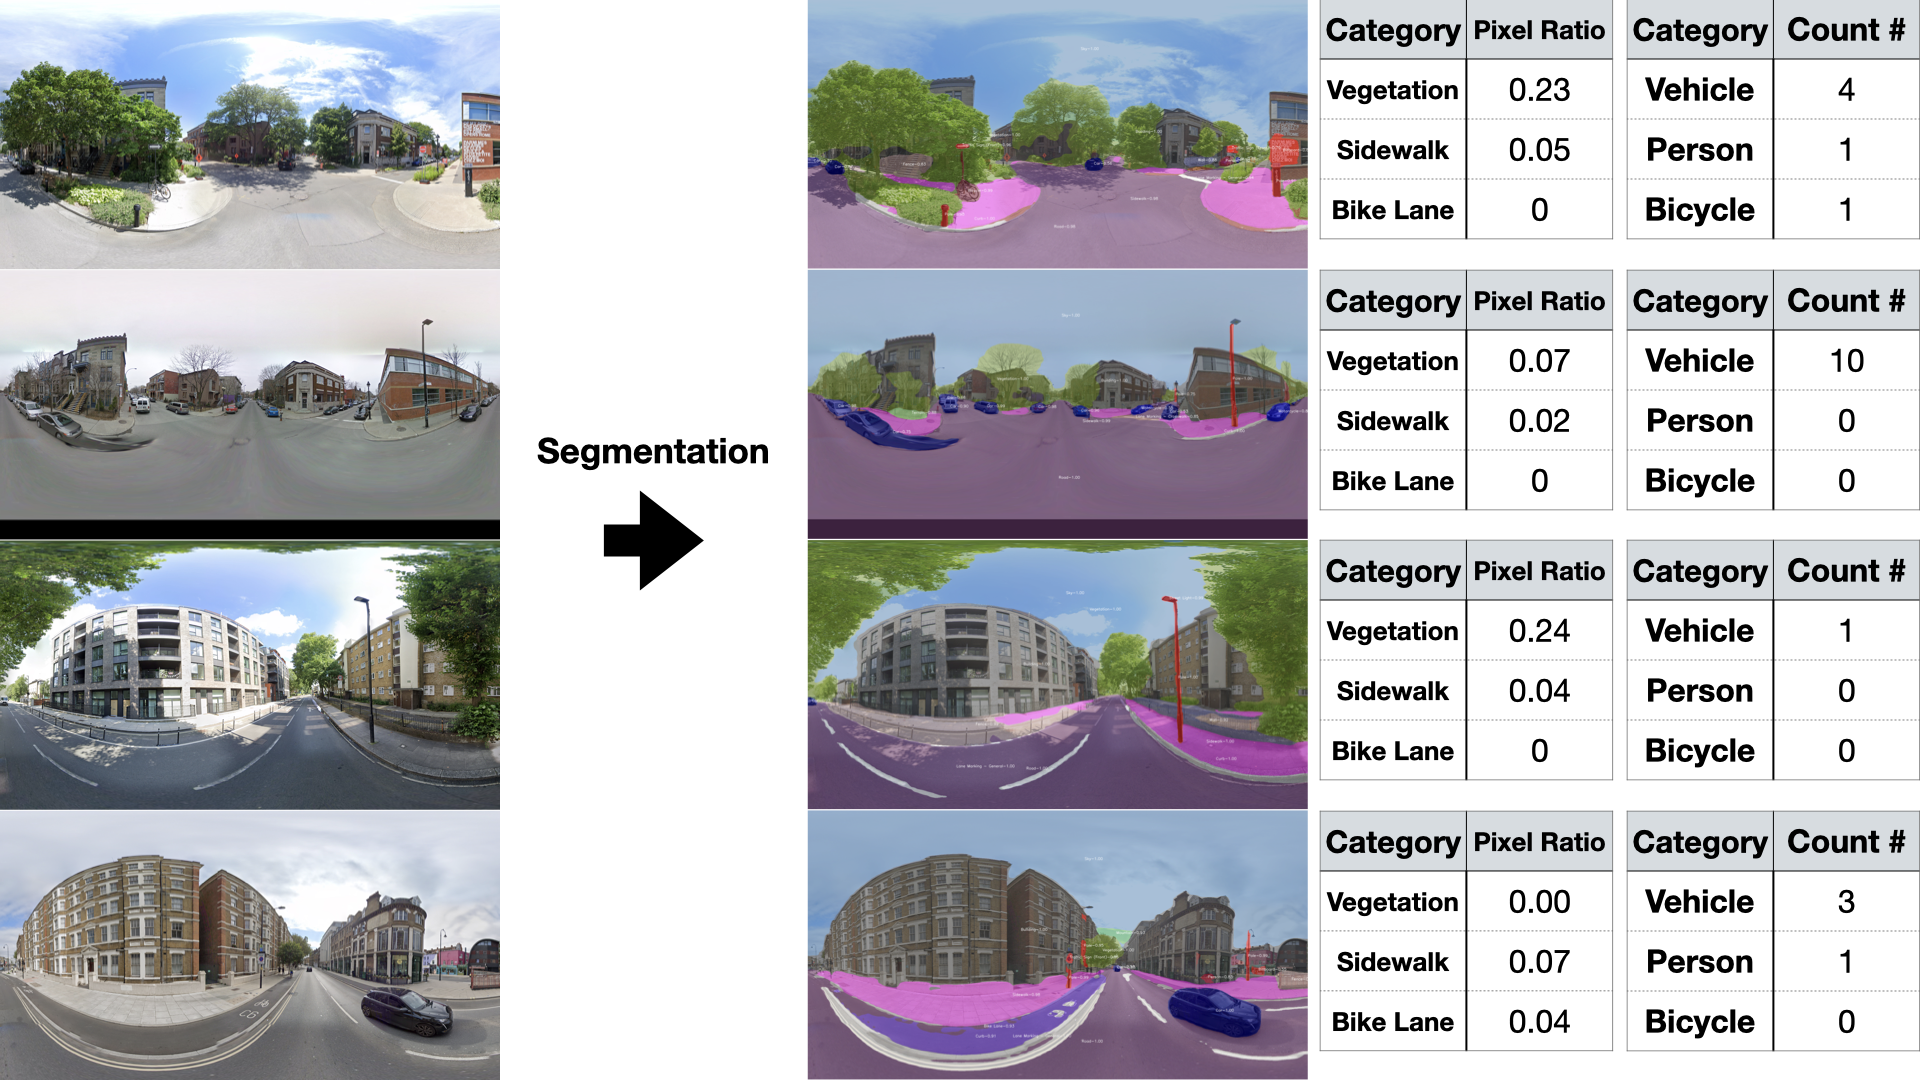
\includegraphics[width=.8\textwidth]{fig/workflow.007.png} 
    \caption{Examples of panoptic segmentation conducted with Mask2Former pre-trained on Mapillary. This process returns both pixel ratios and the count of objects.}
    \label{method:fig:segmentation_example}
\end{figure}

As for spatial variables, the slope in degrees was calculated based on the digital terrain model. We included the average value of slope within 100 meters from each count point as a variable. As for POI data, we utilized the ohsome-py package in Python to retrieve the total number of POIs within 500 meters of the count points each year on January 1 \citep{klonner_sketch_2021}. Lastly, control variables were computed at the census levels (e.g., LSOA in London) and passed to each count point using spatial joining. The importance of the street segment in the street network and POIs was calculated by computing betweenness with POIs as origins and destinations within 1km buffers from the count stations. The accessibility to POIs was calculated as follows:
\begin{align*}
\text{Accessibility} &= \sum_{p \in P} \frac{1}{1 + d_G(n, p)} \\[10pt]
\text{where:} \\
P &= \text{set of all POI nodes within 1km buffer from the count stations} \\
p &= \text{an individual POI node} \\
n &= \text{nearest node to the point of interest} \\
d_G(n, p) &= \text{shortest path length between nodes $n$ and $p$ in graph $G$} \\
G &= \text{street network graph from OpenStreetMap}
\end{align*}

\subsubsection{Propensity Score Matching}
Statistical analysis was performed in three steps: 1. exploratory data analysis, 2. base model construction, and 3. models for causal inference. The first step involved an investigation of two-way correlations among variables. In the second step, we developed step-wise negative binomial models by adding one covariate at a time on top of panel effects to get an initial understanding of the effects of treatments on bikeability. The negative binomial model was selected because overdispersion was observed. Finally, in the third step, two models were estimated to handle the potential confounding biases and analyze the overall and heterogeneous causal effect of the elements of urban design extracted from SVI on the use of active travel modes. As the analysis in the first two steps is fairly standard, this subsection focuses on the specifications of the causal models considered in the third step.  

The first model is a negative binomial (NB) model with year-fixed effects combined with PSM, which is often used to adjust for confounding biases (assuming selection on observed variables) in observational studies and estimate causal effect \citep{zhang_causal_2021}. We added year-fixed effects to capture temporal trends that other variables cannot control for.  

In this study, the PSM model can be expressed as the equation below:
\begin{equation}
\begin{aligned}
Y_i\left(W_i\right) &=Y_i(0) \times\left(1-W_i\right)+Y_i(1) \times W_i \\
Y_i &= \begin{cases}Y_i(0) & \text { if } W_i=0 \\
Y_i(1) & \text { if } W_i=1\end{cases} \\
i &=1, \ldots, N,
\end{aligned}
\end{equation}
where $Y_i$ denotes the number of cyclists counted at observation $i$ among all $N$ observations (i.e. observations at count stations in available years between 2010 and 2019 in London), and $W_i$ represents the binary treatment. Vegetation, sidewalk, and slope were converted to binary variables by partitioning the parameter space at 70 percentiles, and other treatment indicators were converted to binary variables by partitioning at a value of zero (i.e. $W_i=1$ if the treatment indicator is above 0). Thus, the outcome $Y_i$ manifests into $Y_i(0)$ when an observation $i$ is not treated and becomes $Y_i(1)$ when it is treated. The subscript $t$ for the year is suppressed here for the simplicity of notation, as year and month are simply fixed effects in this study.
We binarize the treatment variables, facilitating a direct examination of the effects on cyclist counts. 
While more granular categorization might reveal detailed insights, as demonstrated by previous studies, the binary approach effectively captures significant causal relationships, maintaining the analysis's clarity and accessibility \citep{silva_predicting_2015, frank_build_2021, liu_transitinduced_2023, fosgerau_bikeability_2023, calhoun_estimating_2024}.

The PSM ensures the identification of causal effects under three assumptions.
The first assumption is the conditional independence assumption, which can be expressed as:
\begin{equation}
W_i \perp\left(Y_i(0), Y_i(1)\right) \mid \mathrm{P}\left(X_i\right),
\end{equation}
where $\mathrm{P}\left(X_i\right)$ represents the propensity score of an observation $i$ being treated, given the covariates $X$, such as socioeconomic and land use characteristics in this case.
In this equation, we assume that given the observed covariates (encapsulated in $\mathrm{P}\left(X_i\right)$), the assignment of treatment (e.g., vegetation and slope) is independent of the potential outcomes (i.e. number of counted cyclists).

The second assumption is the common support assumption in the covariate distributions when separated by treatment status. 
This assumption can be written as:
\begin{equation}
0<P\left(W_i=1 \mid X_i=x\right)<1 \quad \text { for all } x,
\end{equation}
where $P\left(W_i=1 \mid X_i=x\right)$ is the probability (i.e. propensity score) of being treated for observation $i$ given the covariate vector $X_i$ takes a value of $x$. 
The propensity scores of both treated (i.e. $W_i=1$) and non-treated (i.e. $W_i=0$) observations need to overlap over the entire domain of $X$ to satisfy the assumption. We test this assumption in this study. 

The last assumption is the stable unit treatment value assumption, which requires the outcome for each observation to be independent of the treatment status of other observations. There is no specific reason for the violation of this assumption in this study. As the treatments were converted to binary variables in this study, this assumption can be expressed as:
\begin{equation}
Y_i=W_i Y_i(1)+\left(1-W_i\right) Y_i(0)
\end{equation}

In our study, the propensity score was calculated based on the logistic regression model as follows:
\begin{equation}
P(W_i=1) = \frac{\mathrm{e}^{\left(\beta_0 + \beta_l \times X_i\right)}}{1+\mathrm{e}^{\left(\beta_0 + \beta_l \times X_i\right)}},
\end{equation}
where $P$ represents the propensity score, and $\beta$ denotes the coefficients for covariate vector $X_i$. 
We conducted full matching using the R package \texttt{MatchIt} by \citet{ho_matchit_2011}. Unlike traditional 1:1 or 1:k matching, full matching creates subclasses in which both treated and control units have similar propensity scores. The subclasses can be described as follows:

\begin{equation}
\begin{aligned}
\text{Subclass } S_j = \{ m,n \} \mid |P_m - P_n| < \epsilon
\end{aligned}
\end{equation}

where:
\begin{itemize}
    \item \( S_j \) is the \( j^{th} \) subclass.
    \item \( m \) belongs to the treated units and \( n \) belongs to the control units.
    \item \( P_m \) and \( P_n \) are the propensity scores of treated unit \( m \) and control unit \( n \), respectively.
    \item \( \epsilon \) is a small threshold value that ensures that units within the subclass have propensity scores within \( \epsilon \) of each other.
\end{itemize}
The treatment effect is then estimated by averaging the differences in the outcomes within all subclasses.

After matching treated and control units, we constructed an NB model with the following equation by calculating the probability of \(Y_i= y_i\) :
\begin{equation}
\begin{aligned}
Pr\left(Y_i=y_i\right)&=
\frac{\Gamma\left(y_i+\frac{1}{\tau}\right)}{\Gamma\left(\frac{1}{\tau}\right) y_i!}\left(\frac{1}{1+\tau \mu_i}\right)^{\frac{1}{\tau}}\left(\frac{\tau \mu_i}{1+\tau \mu_i}\right)^{y_i}, \\
y_i&=0,1,2,3, \ldots,
\end{aligned}
\end{equation}
where \(y_i\), the number of cyclists counted at a station in a specific year, is assumed to follow the negative binomial distribution with mean \(\mu_i\) and dispersion coefficient \(\tau\).

\(\mu_i\) can be defined and transformed as:
\begin{equation}
\begin{aligned}
\mu_{i} &=\exp \left(\boldsymbol{X}_{\boldsymbol{i}}^T \boldsymbol{\gamma}\right) \\
\ln \hat{\mu_{i}} &=\hat{\gamma}_0+\sum_{j=1}^k \hat{\gamma_j} X_{i j}
\end{aligned}
\end{equation}
where \(X\) denotes the predictor variables (i.e. the treatment variable and covariates), \(\gamma\) represents the coefficients for the negative binomial model, and \(k\) is the number of predictor variables \citep{ashqar_modeling_2019}.

The model for \(\ln \hat{\mu_i}\) is the negative binomial model to predict the cyclist count.

Finally, the average treatment effects (ATE) can be estimated as:
\begin{equation}
\widehat{\mathrm{ATE}} = \left( \frac{1}{N} \sum_{i=1}^N W_i \ln \hat{\mu_{i}} \right) - \left( \frac{1}{N} \sum_{i=1}^N (1-W_i) \ln \hat{\mu_{i}} \right),
\end{equation}
where \(N\) denotes the number of units; thus the left half of the equation (i.e. \(\frac{1}{N} \sum_{i=1}^N W_i \ln \hat{\mu_{i}}\)) is the average predicted log counts of the outcome \(\mu_{i}\) among the treated units with the weight of 1.
The right half of the equation is the average among the matched control units.

\subsubsection{Causal Forest}
The other model is the causal forest proposed by \citet{athey_estimating_2019}. 
This model estimates conditional average treatment effects (CATE), which inform the average treatment effects under certain conditions of covariates, which can be expressed as:
\begin{equation}
\tau(x)=\mathbb{E}\left[Y_i(1)-Y_i(0) \mid X_i=x\right],
\end{equation}
where $\tau(x)$ denotes CATE given covariates $X_i$. 
However, one cannot observe $Y_i(1)$ and $Y_i(0)$ at the same time.
To overcome this challenge, a causal forest model, which consists of causal trees, obtains CATE by calculating the difference between the outcomes of treated and control units within the same leaf based on the assumption that a leaf is small enough to achieve unconfoundedness.
Such causal trees can be expressed as:
\begin{equation}
\begin{aligned}
\hat{\tau}(x)= & \frac{1}{\left|\left\{i: W_i=1, X_i \in L\right\}\right|} \sum_{\left\{i: W_i=1, X_i \in L\right\}}^{Y_i} \\
& -\frac{1}{\left|\left\{i: W_i=0, X_i \in L\right\}\right|} \sum_{\left\{i: W_i=0, X_i \in L\right\}}^{Y_i},
\end{aligned}
\label{methodology:equation:causal_tree}
\end{equation}
where $L$ represents a leaf in a decision tree, and $i$ denotes indices for observations in the leaf $L$. 
Intuitively, it is a kind of non-parametric PSM approach, which makes covariate $X$ similar enough within the same leaf between treatment and control observation such that the treatment assignment becomes a random assignment. 
Such a concept of a causal tree was exemplified by visualizing a simple diagram in \autoref{method:fig:ct_example}, and each leaf is represented as a purple box, within which comparisons of $Y_i$ between $W_i = 1$ and $W_i = 0$ can return treatment effects with unconfoundedness. 
In other words, \autoref{methodology:equation:causal_tree} sums the outcomes $Y_i$ for each of two groups (i.e., $W_i = 1$ and $W_i = 0$) separately and computes their averages within $L$. This method isolates the treatment effect by ensuring comparisons are made between similar observations.

\begin{figure}[!htp]
    \centering
    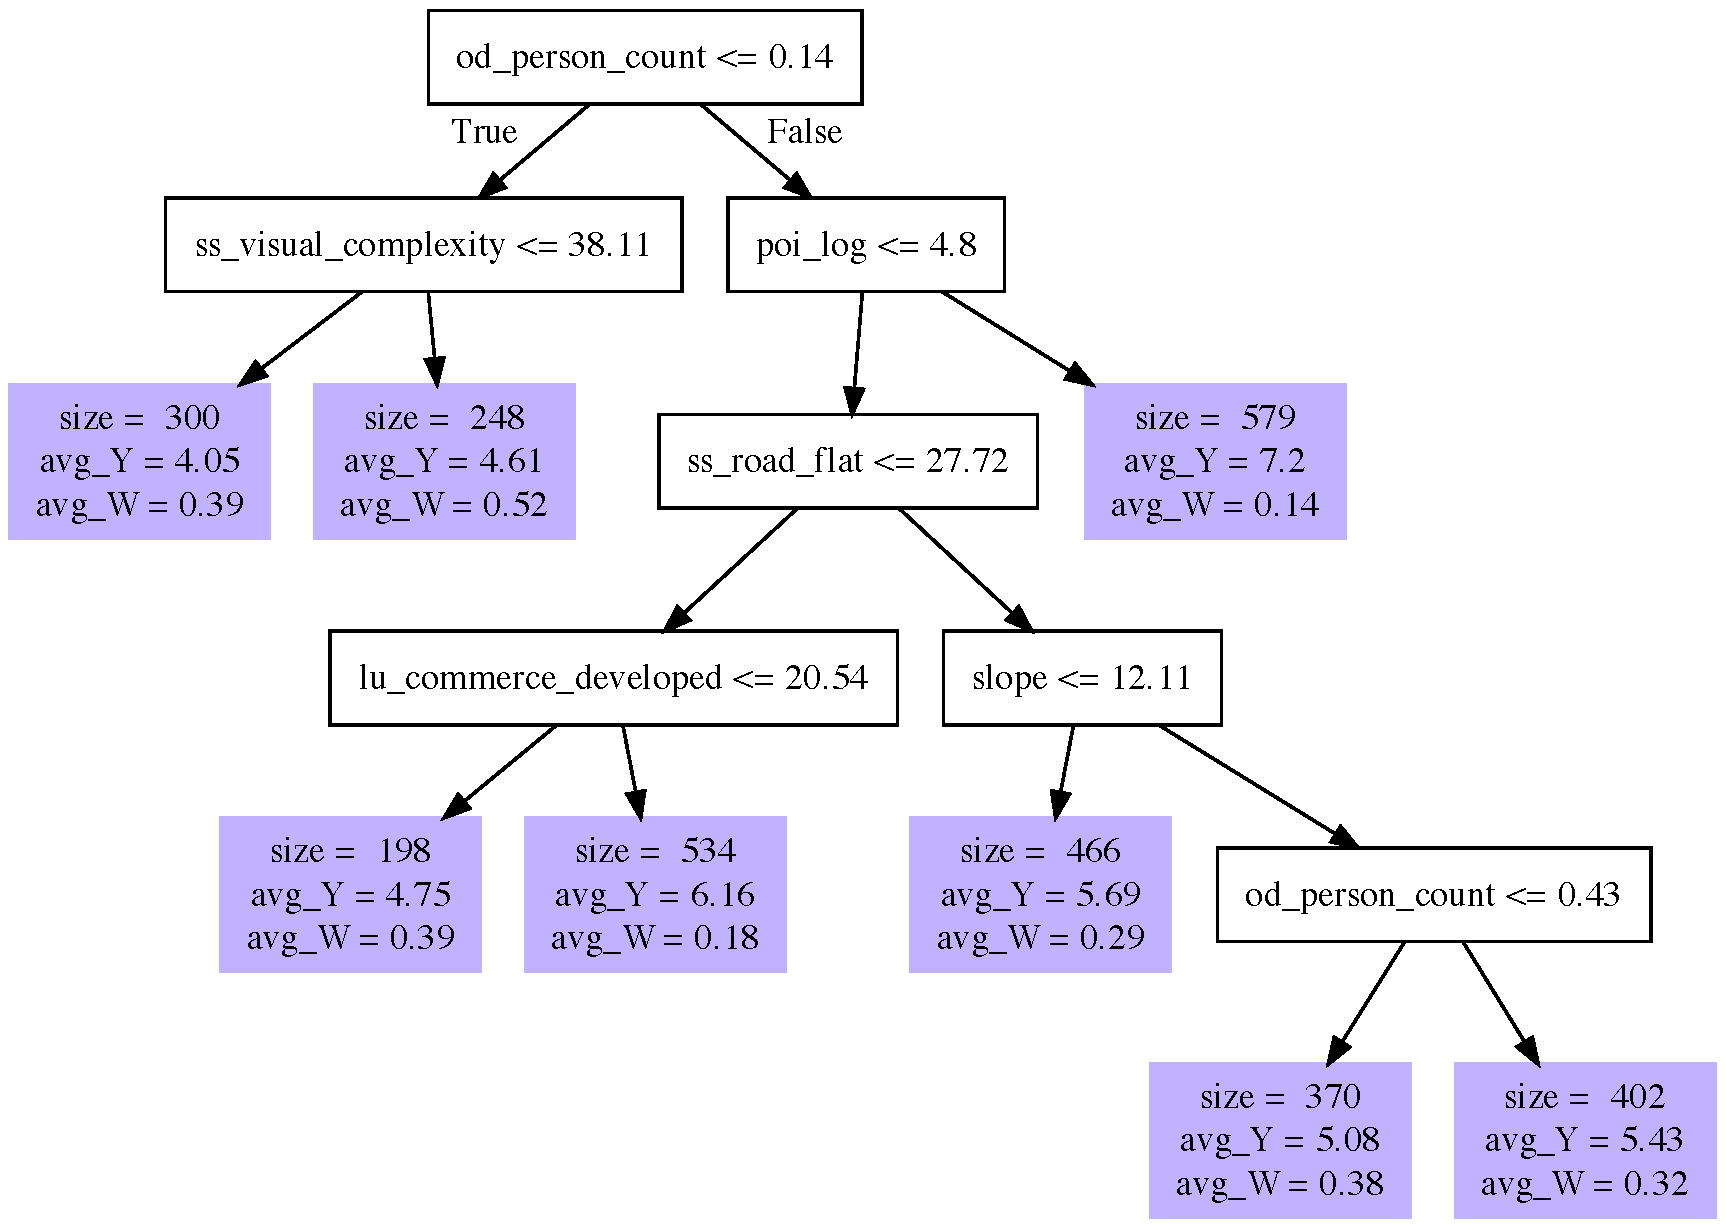
\includegraphics[width=.8\textwidth]{fig/binary_ss_vegetation_binary_causal_tree.pdf} 
    \caption{An example of a causal tree.}
    \label{method:fig:ct_example}
\end{figure}

For this study, we used grf --- an R package developed by \citet{athey_generalized_2019}.
Additionally, we estimate conditional average treatment effects (CATE) units to compare them with the ATE estimated using PSM at an aggregated level. We estimated CATE using the following steps:
\begin{enumerate}
    \item \textbf{Training Regression Forests for Propensity Score and Marginal Outcomes}:
    \begin{itemize}
        \item We initiate the process with regression forests to predict the propensity score $e(x)=\mathbb{E}\left[W \mid X=x\right]$ and marginal outcomes $m(x) = \mathbb{E}\left[Y \mid X=x\right]$. These models estimate, respectively, the likelihood of receiving treatment based on unit characteristics and the expected outcome, using the out-of-bag prediction method for unbiased estimates.
    \end{itemize}

    \item \textbf{Training Causal Forests on Residuals}:
    \begin{itemize}
        \item A causal forest is then trained on the residuals: the treatment $W - e(x)$ and outcome $Y - m(x)$ residuals. This approach focuses on isolating the treatment's effect by analyzing the variance between actual and predicted values, utilizing double-sample trees to maximize and estimate treatment effects within distinct groups or leaves.
    \end{itemize}

    \item \textbf{Estimating the Treatment Effect}:
    \begin{equation}
    \hat{\tau}=\frac{\sum_i \alpha_i(x)\left(Y_i-\hat{m}^{(-i)}\left(X_i\right)\right)\left(W_i-\hat{e}^{(-i)}\left(X_i\right)\right)}{\sum_i \alpha_i(x)\left(W_i-\hat{e}^{(-i)}\left(X_i\right)\right)^2},
    \end{equation}
    \begin{itemize}
        \item The treatment effect $\hat{\tau}$ is estimated by weighing the outcome differences within groups, corrected by the propensity score, to ensure a like-for-like comparison and reliable treatment impact estimation.
    \end{itemize}

    \item \textbf{Estimating CATE Using a Doubly Robust Method}:
    \begin{equation}
    \begin{aligned}
    \widehat{C A T E} & =\frac{1}{n} \sum_{i=1}^n \left\{ \hat{\tau}^{(-i)}\left(X_i\right) + \frac{W_i-\hat{e}^{(-i)}\left(X_i\right)}{\hat{e}^{(-i)}\left(X_i\right)\left(1-\hat{e}^{(-i)}\left(X_i\right)\right)} \left[ Y_i-\hat{m}^{(-i)}\left(X_i\right) \right. \right. \\
    & \left. \left. -\left(W_i-\hat{e}^{(-i)}\left(X_i\right)\right) \hat{\tau}^{(-i)}\left(X_i\right) \right] \right\}
    \end{aligned}
    \end{equation}
    \begin{itemize}
        \item This step refines the CATE estimation for cyclist counts with the doubly robust AIPW estimator, combining propensity score and causal forest predictions to correct biases and enhance accuracy.
    \end{itemize}
\end{enumerate}


The causal forest model inherits the strengths from traditional statistics and machine learning \citep{athey_estimating_2019}. Its strengths over traditional parametric models with linear link function are:
\begin{itemize}
    \item It provides heterogeneous causal effects, obviating the need to specify interaction terms apriori. Its improved functional flexibility allows for complex nonlinear and interactive effects of explanatory variables, thereby reducing the bias caused by model misspecification.
    \item It can complement the weakness of PSM --- potential risk of increasing imbalance, inefficiency, and bias by discarding unmatched units \citep{ripollone_implications_2018, guo_propensity_2020}. Some of these issues can also be overcome with inverse probability weighting, but it is more prone to misspecifications; thus, the causal forest's non-parametric feature helps address these issues comprehensively. 
\end{itemize}
And its strengths over non-causal machine learning models are:
\begin{itemize}
    \item While other machine learning models, such as random forest, are designed to maximize predictive accuracy, the causal forest is designed to maximize heterogeneity and use covariates to control for confounders, thereby discovering causal effects.
    \item Causal forest's estimates are consistent and asymptotically normal, meaning that we can get valid confidence intervals for the treatment effects.
\end{itemize}

Due to these reasons, we chose a causal forest to estimate heterogeneous causal effects in this study. Despite its advantages, previous research in bikeability has not fully utilized this model.

\section{Results and discussion} \label{sc:result}
\subsection{Correlation Analysis}
\autoref{result:tab:variables} explains the variables in the collected data.
Correlation matrix plots were created to investigate the two-way relationships between variables without controlling for any other variables (\autoref{result:fig:corr_mat}). The plot shows that the built environment characteristics have correlations with the cyclist count --- $count$; for example, $ss\_construction$ (i.e. human-built objects such as buildings) have positive correlations, while vehicle-related variables such as $ss\_road\_flat$ and $od\_vehicle\_count$ have negative correlations. 
Other visual elements, such as human-related variables (e.g., $od\_person\_count$), are also positively correlated with the count of cyclists, which is aligned with intuition. 
Other socioeconomic variables such as $age\_0\_19$ and $age\_20\_39$ composition also have correlations, and $poi\_log$, $housing\_price\_log$, $lu\_commerce\_developed$, and $poi\_accessibility\_log$ have strong correlations as well.

Acknowledging that there is no control variable in this pair-wise correlation analysis, it is interesting that vegetation has negative correlations with the number of cyclists, which is in contrast to the findings in the literature \citep{bai_how_2022, chen_eyelevel_2020}. This is possibly due to the concentration of higher counts in the central business district areas while higher pixel ratios of vegetation are found in the surrounding areas.

\begin{table}[!ht]\centering
\caption{Variables used in this study with Spatial Scale.}\label{result:tab:variables}
\tiny
\begin{tabular}{lrr}\toprule
Variables & Meaning & Spatial Scale \\\midrule
count & Dependent variables: average daily count of cyclists at a monthly level & \\
 & collected by Transport for London from years 2010 to 2019 & \\
year & Year of the observation as a fixed effect & \\
month & Month of the observation as a fixed effect & \\
ss\_sidewalk & Ratio of pixel segmented as sidewalk & 100m buffer (mean) \\
ss\_vegetation & Ratio of pixel segmented as vegetation & 100m buffer (mean) \\
ss\_guard\_rail & Ratio of pixel segmented as guard rails & 100m buffer (mean) \\
 & (i.e., safety barriers separating pedestrians from vehicles) & \\
ss\_street\_light & Ratio of pixel segmented as street light & 100m buffer (mean) \\
ss\_parking & Ratio of pixel segmented as parking & 100m buffer (mean) \\
ss\_bike\_lane & Ratio of pixel segmented as bike lane & 100m buffer (mean) \\
ss\_construction & Ratio of pixel segmented as fence, barrier, wall, bridge, & 100m buffer (mean) \\
 & building, or tunnel & \\
ss\_road\_flat & Ratio of pixel segmented as road, crosswalk, rail track, & 100m buffer (mean) \\
 & or service lane & \\
ss\_marking & Ratio of pixel segmented as crosswalk marking or general & 100m buffer (mean) \\
 & lane marking & \\
ss\_nature & Ratio of pixel segmented as mountain, sand, snow, terrain, & 100m buffer (mean) \\
 & or water & \\
ss\_street\_object & Ratio of pixel segmented as banner, billboard, catch basin, & 100m buffer (mean) \\
 & CCTV camera, fire hydrant, junction box, mailbox, manhole, & \\
 & phone booth, poles, traffic sign/light, or trash can & \\
ss\_visual\_complexity & Visual complexity & 100m buffer (mean) \\
od\_person\_count & Count of person detected by object detection from SVI & 100m buffer (mean) \\
od\_bicycle\_count & Count of bicycle detected by object detection from SVI & 100m buffer (mean) \\
od\_vehicle\_count & Count of vehicle detected by object detection from SVI & 100m buffer (mean) \\
od\_animal\_count & Count of animal detected by object detection from SVI & 100m buffer (mean) \\
pop\_den\_log & Log-transformed population density (km$^2$) & Extracted from census data \\
average\_income\_log & Log-transformed average income & Extracted from census data \\
housing\_price\_log & Log-transformed average housing price & Extracted from census data \\
poi\_log & Log-transformed count of POI & 500m buffer (sum) \\
age\_0\_19 & Ratio of population between 0 and 19 & Extracted from census data \\
age\_20\_39 & Ratio of population between 20 and 39 & Extracted from census data \\
age\_40\_59 & Ratio of population between 40 and 59 & Extracted from census data \\
IMD\_score & Indices of Multiple Deprivation & Extracted from census data \\
lu\_residential\_community & Share of residential and community service (land use) & Extracted from census data \\
lu\_commerce\_developped & Share of commercial, industry, transport, and & Extracted from census data \\
 & unknown developed use (land use) & \\
slope & Average slope in 100m buffer & 100m buffer (mean) \\
poi\_betweenness\_log & Log-transformed betweenness of street segments from and to POIs within 1km buffers & nearest street node \\
poi\_accessibility\_log & Log-transformed accessibility to POIs & nearest street node \\
traffic\_speed\_log & Log-transformed traffic speed limit & nearest street node \\

\bottomrule
\end{tabular}
\end{table}

\begin{figure}
    \centering
    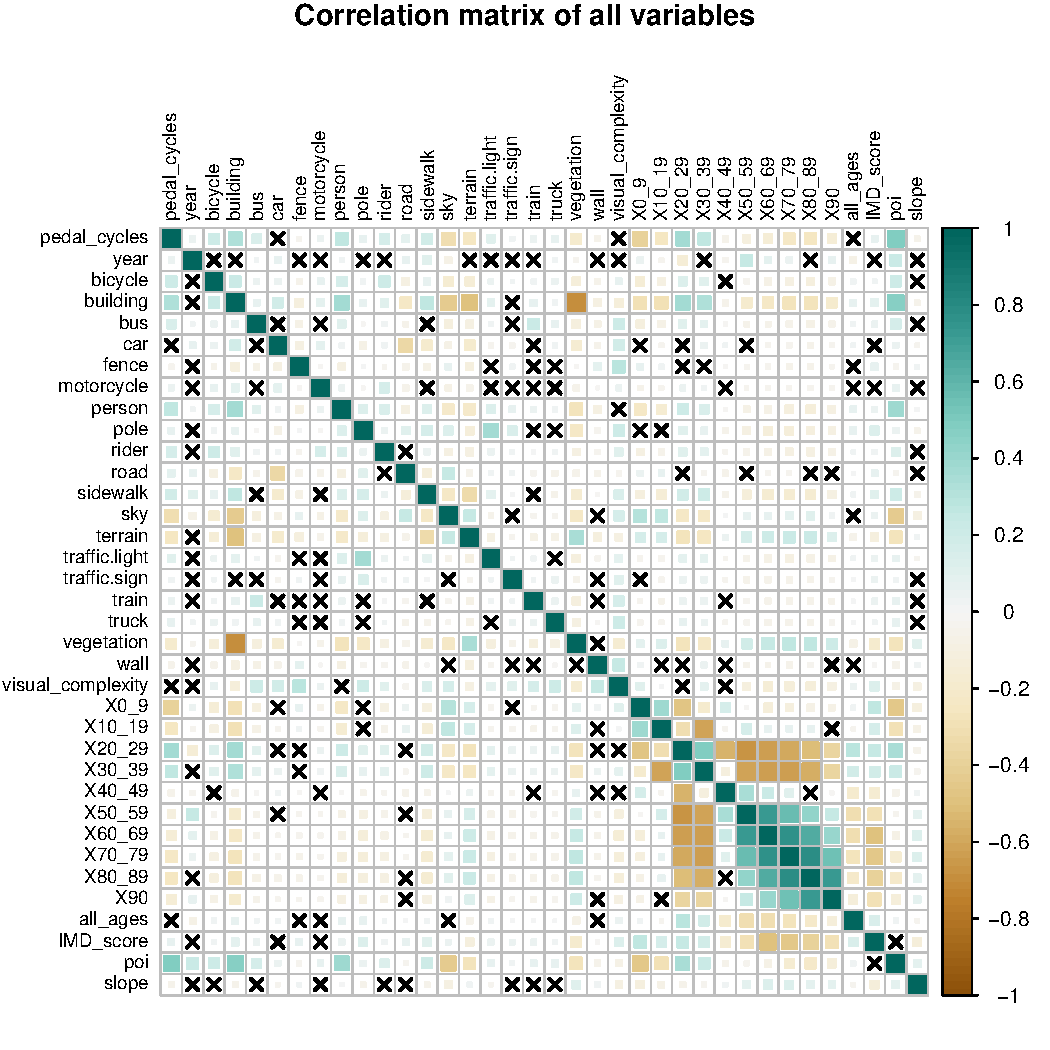
\includegraphics[width=\textwidth]{fig/London/correlation_mat.pdf}
    \caption{Correlation matrix plot of all the variables in this study. Being crossed means that there is no statistical significance (i.e. p-value above 0.05). We aggregated the data across all the years.}
    \label{result:fig:corr_mat}
\end{figure}

\subsection{Negative Binomial Model}
Based on the insights derived from the correlational analysis, we constructed step-wise count data models with year-fixed effects and socioeconomic controls (e.g., year, month, age group composition, and land use) to evaluate the sensitivity of the effect of treatment indicators on bicycle counts relative to the addition of different covariates to the baseline specification.
We investigated the over-dispersion of the data by building Poisson models and running a statistical test, which returned an alpha value of around 800 with a p-value lower than 0.001, indicating the over-dispersion. 
Therefore, the NB model was selected over the Poisson regression model. 
Additionally, we also conducted a variance inflation factor (VIF) test to confirm the absence of strong multicollinearity (i.e., VIF>5.0).

\autoref{result:fig:step_model_part1} and \autoref{result:fig:step_model_part2} show bar plots of point estimates (i.e. purple bars) and p-values (i.e. green bars) associated with the effect of treatment indicators on bicycle counts, resulting from negative binomial specification where different covariates are added into the baseline model. 
Most treatment indicators have steady estimates, either positive (e.g., bike lane) or negative (e.g., slope), but street parking had higher p-values and fluctuating point estimates. 
Such fluctuations can be explained by a few reasons, including but not limited to weak effects of the treatment variables and some degree of correlations among the dependent variables, treatment variables, and covariates. 
Street parking has higher p-values for most of the added covariates, suggesting that its effects are potentially weak and can be easily affected by covariates.
Correlations among variables might have caused fluctuations in cases such as the high p-value of bike lanes with POIs.

\begin{figure}
    \centering
    \begin{subfigure}{0.7\textwidth}
        \centering
        \includegraphics[width=\linewidth]{fig/London/vegetation/no_title_year_negative_binomial_result.png}
        \caption{Vegetation}
    \end{subfigure}
    
    \vspace{1cm} % Add some vertical space between subfigures
    
    \begin{subfigure}{0.7\textwidth}
        \centering
        \includegraphics[width=\linewidth]{fig/London/slope/no_title_year_negative_binomial_result.png}
        \caption{Slope}
    \end{subfigure}
    \caption{Results of step-wise negative binomial models for treatment variables. Plots show the results of vegetation and slope. The purple bars represent the point estimates of the treatment variables when we added the variable shown on the x-axis, and the green bars represent their p-values.}
    \label{result:fig:step_model_part1}
\end{figure}

\begin{figure}
    \centering
    \begin{subfigure}{0.7\textwidth}
        \centering
        \includegraphics[width=\linewidth]{fig/London/bike_lane/no_title_year_negative_binomial_result.png}
        \caption{Bike Lane}
    \end{subfigure}
    
    \vspace{1cm} % Add some vertical space between subfigures
    
    \begin{subfigure}{0.7\textwidth}
        \centering
        \includegraphics[width=\linewidth]{fig/London/parking/no_title_year_negative_binomial_result.png}
        \caption{Parking}
    \end{subfigure}
    
    \vspace{1cm} % Add some vertical space between subfigures
    
    \begin{subfigure}{0.7\textwidth}
        \centering
        \includegraphics[width=\linewidth]{fig/London/street_light/no_title_year_negative_binomial_result.png}
        \caption{Street Light}
    \end{subfigure}
    
    \caption{Results of step-wise negative binomial models for treatment variables. Plots show results of bike lanes, parking, and street lights. The purple bars represent the point estimates of the treatment variables when we added the variable shown on the x-axis, and the green bars represent their p-values.}
    \label{result:fig:step_model_part2}
\end{figure}

\subsection{Negative Binomial Model with Propensity Score Matching}
After the data exploration and initial modeling, NB with PSM was estimated. 
One of the assumptions of PSM is common support, which can be checked by observing the propensity score distribution of both treated and non-treated observations. We visualized the propensity scores of the control and treatment groups with histograms in \autoref{result:fig:psm}.
Most plots show that the distribution of propensity scores of treated units (i.e. green parts) and control units (i.e. gray parts) have overlapping areas, thereby satisfying the common support assumption. 

After checking the data balance, we estimated the first-stage PSM model (i.e. logit models to compute propensity scores) (see \autoref{result:tab:psm_stage1_london}). We included all variables following the findings of \citet{brookhart_variable_2006, zhang_propensity_2021}, who reported that the inclusion of such covariates can improve the performance of the model regardless of whether they affect the assignment of treatment. Since it is a predictive model, we do not delve deeper into the statistical significance of parameter estimates. 

\begin{table}[!htbp]
\centering 
  \caption{This table shows the results (i.e. ATE) of second-stage negative binomial models of PSM for cyclists counts in London. Standard errors are in parenthesis.} 
  \label{result:tab:psm_stage2_london} 
\scriptsize
\begin{tabular}{@{\extracolsep{1pt}}lccccc} 
\toprule 
 & \multicolumn{5}{c}{\textit{Dependent variable:}} \\ 
\cmidrule{2-6} 
 & \multicolumn{5}{c}{count} \\ 
 & vegetation & bike lane & parking & street light & slope\\ 
\midrule 
  Treatment variables & 0.133$^{*}$ (0.079) & 0.611$^{***}$ (0.133) & 0.208$^{*}$ (0.120) & 0.018 (0.069) & $-$0.332$^{***}$ (0.073) \\ 
Observations & 1,274 & 1,274 & 1,274 & 1,274 & 1,274 \\ 
Log Likelihood & $-$7,479.289 & $-$7,637.008 & $-$7,791.420 & $-$7,663.579 & $-$7,653.867 \\ 
$\theta$ & 0.646$^{***}$  (0.024) & 0.712$^{***}$  (0.026) & 0.727$^{***}$  (0.026) & 0.712$^{***}$  (0.026) & 0.717$^{***}$  (0.026) \\ 
Akaike Inf. Crit. & 15,036.580 & 15,352.020 & 15,660.840 & 15,405.160 & 15,383.740 \\ 
\bottomrule 
\addlinespace[.5ex]
\multicolumn{6}{l}{\textit{Note:}  $^{*}$p$<$0.1; $^{**}$p$<$0.05; $^{***}$p$<$0.01} \\ 
\end{tabular} 
\end{table}

% Table created by stargazer v.5.2.3 by Marek Hlavac, Social Policy Institute. E-mail: marek.hlavac at gmail.com
% Date and time: Wed, Aug 09, 2023 - 17:56:24
\begin{table}[!htbp]
\centering
\caption{This table shows the results of the first stage logit models in the PSM for London.}
\label{result:tab:psm_stage1_london}
\resizebox{\textwidth}{!}{%
\scriptsize
\begin{tabular}{@{\extracolsep{1pt}}lccccc}
\toprule
 & \multicolumn{5}{c}{\textit{Dependent variable:}} \\
\cline{2-6}
\\[-1.8ex] & ss\_vegetation\_binary & ss\_bike\_lane\_binary & ss\_parking\_binary & ss\_street\_light\_binary & slope\_binary \\
\\[-1.8ex] & (1) & (2) & (3) & (4) & (5)\\
\midrule
 year2011 & $-$11.876 (2,345.862) & 0.023 (1,495.464) & $-$0.295 (1,232.047) & 14.495 (432.246) & $-$0.770 (1.490) \\
  year2012 & $-$0.161 (12.798) & 13.480 (1,267.442) & 12.122 (1,032.133) & 13.733 (432.245) & 0.138 (1.215) \\
  year2014 & $-$0.262 (12.804) & 12.959 (1,267.442) & 13.020 (1,032.133) & 13.543 (432.245) & $-$0.213 (1.217) \\
  year2015 & $-$0.234 (12.784) & 12.533 (1,267.442) & 12.333 (1,032.133) & 13.486 (432.245) & $-$0.626 (1.212) \\
  year2016 & $-$0.605 (12.841) & 11.523 (1,267.442) & 12.979 (1,032.133) & 13.179 (432.245) & $-$0.459 (1.228) \\
  year2017 & $-$0.320 (12.808) & 12.660 (1,267.442) & 12.209 (1,032.133) & 13.405 (432.245) & $-$0.610 (1.223) \\
  year2018 & 2.089 (12.847) & 13.863 (1,267.442) & 15.017 (1,032.133) & 14.945 (432.245) & $-$0.820 (1.239) \\
  year2019 & 2.240 (12.779) & 14.152 (1,267.442) & 14.675 (1,032.133) & 14.360 (432.245) & $-$0.817 (1.214) \\
  month4 & 0.201 (2.096) & $-$0.357 (0.548) & $-$0.905$^{**}$ (0.441) & $-$0.525 (0.366) & $-$0.090 (0.401) \\
  month5 & $-$0.152 (1.832) & $-$0.879$^{*}$ (0.529) & $-$0.535 (0.361) & $-$0.742$^{**}$ (0.320) & 0.170 (0.344) \\
  month6 & $-$0.356 (1.861) & 0.176 (0.494) & $-$0.540 (0.368) & $-$0.340 (0.323) & 0.430 (0.347) \\
  month7 & $-$0.315 (2.070) & $-$0.664 (0.616) & $-$0.637 (0.442) & $-$0.668$^{*}$ (0.358) & 0.153 (0.383) \\
  month9 & $-$0.866 (2.169) & $-$0.290 (0.669) & $-$0.483 (0.481) & $-$0.728$^{**}$ (0.363) & 0.137 (0.386) \\
  month10 & 0.189 (2.080) & $-$0.920 (0.758) & $-$0.612 (0.502) & $-$0.943$^{**}$ (0.367) & 0.101 (0.385) \\
  month11 & $-$15.074 (11,392.340) & $-$14.269 (2,639.256) & $-$13.801 (2,179.277) & $-$14.570 (912.128) & $-$12.056 (330.961) \\
  slope & 0.006 (0.057) & $-$0.019 (0.023) & $-$0.016 (0.017) & $-$0.021$^{**}$ (0.010) &  \\
  IMD\_score & 0.002 (0.047) & $-$0.0001 (0.017) & 0.032$^{***}$ (0.012) & 0.011 (0.008) & $-$0.006 (0.009) \\
  age\_0\_19 & $-$0.023 (0.106) & $-$0.041 (0.039) & 0.022 (0.030) & $-$0.034$^{*}$ (0.019) & 0.0004 (0.019) \\
  age\_20\_39 & $-$0.005 (0.080) & 0.030 (0.030) & 0.025 (0.024) & $-$0.004 (0.014) & 0.003 (0.014) \\
  age\_40\_59 & 0.054 (0.158) & 0.045 (0.059) & 0.040 (0.046) & 0.006 (0.028) & $-$0.002 (0.029) \\
  lu\_residential\_community & 0.004 (0.054) & 0.004 (0.020) & $-$0.007 (0.016) & 0.013 (0.010) & $-$0.006 (0.010) \\
  lu\_commerce\_developed & $-$0.009 (0.043) & $-$0.004 (0.015) & 0.002 (0.011) & $-$0.007 (0.007) & $-$0.010 (0.007) \\
  ss\_visual\_complexity & 0.300 (0.192) & 0.072 (0.062) & 0.134$^{***}$ (0.049) & 0.083$^{***}$ (0.027) & $-$0.030 (0.022) \\
  ss\_construction & $-$0.330$^{**}$ (0.134) & $-$0.011 (0.028) & 0.055$^{***}$ (0.021) & 0.031$^{**}$ (0.014) & 0.004 (0.014) \\
  ss\_road\_flat & $-$0.102 (0.113) & 0.038 (0.038) & 0.00001 (0.028) & $-$0.005 (0.016) & 0.016 (0.015) \\
  ss\_marking & $-$0.208 (0.263) & 0.042 (0.068) & $-$0.148$^{*}$ (0.089) & $-$0.075$^{*}$ (0.043) & $-$0.033 (0.043) \\
  ss\_nature & $-$0.057 (0.178) & 0.019 (0.076) & $-$0.078 (0.096) & 0.021 (0.029) & 0.078$^{***}$ (0.029) \\
  ss\_street\_object & $-$2.691 (2.003) & 0.633 (0.425) & $-$1.098$^{**}$ (0.440) & 1.096$^{***}$ (0.269) & 0.084 (0.269) \\
  od\_person\_count & 0.043 (0.755) & 0.037 (0.218) & $-$0.076 (0.179) & $-$0.157 (0.122) & 0.180 (0.120) \\
  od\_vehicle\_count & $-$0.315$^{*}$ (0.186) & $-$0.165$^{**}$ (0.068) & 0.259$^{***}$ (0.047) & $-$0.042 (0.030) & 0.009 (0.030) \\
  od\_animal\_count & 1.660 (26.437) & $-$2.358 (5.751) & $-$27.143 (19.034) & $-$7.936 (7.576) & $-$0.386 (3.009) \\
  housing\_price\_log & 0.484 (1.119) & $-$0.327 (0.419) & 0.380 (0.315) & $-$0.286 (0.197) & 0.674$^{***}$ (0.194) \\
  poi\_betweenness\_log & 0.068 (0.163) & 0.021 (0.051) & $-$0.037 (0.039) & $-$0.011 (0.027) & $-$0.094$^{***}$ (0.029) \\
  poi\_accessibility\_log & 0.160 (0.800) & $-$0.015 (0.309) & $-$0.008 (0.227) & 0.240$^{*}$ (0.140) & $-$0.049 (0.144) \\
  nearest\_edge\_speed\_kph\_log & $-$0.572 (1.955) & 0.882 (0.807) & $-$0.495 (0.610) & 0.285 (0.355) & 1.497$^{***}$ (0.378) \\
  pop\_den\_log & $-$0.067 (0.599) & 0.303 (0.222) & 0.107 (0.172) & 0.020 (0.096) & 0.091 (0.098) \\
  poi\_log & 0.294 (0.573) & 0.282 (0.198) & 0.110 (0.152) & $-$0.057 (0.095) & 0.276$^{***}$ (0.100) \\
  Constant & $-$9.703 (24.529) & $-$22.370 (1,267.467) & $-$29.228 (1,032.151) & $-$14.013 (432.260) & $-$15.227$^{***}$ (3.784) \\
\midrule
Observations & 1,274 & 1,274 & 1,274 & 1,274 & 1,274 \\
\bottomrule
\multicolumn{6}{r}{\textit{Note:} $^{*}$p$<$0.1; $^{**}$p$<$0.05; $^{***}$p$<$0.01} \\
\end{tabular}
}
\end{table}

After matching treated units with the nearest control units in terms of propensity scores, negative binomial models were estimated. The results are displayed in \autoref{result:tab:psm_stage2_london}.
Vegetation, bike lanes, and street parking have a significantly positive ATE on the count of cyclists, and the slope has a significantly negative effect. 
Street lights have a positive effect but it is not statistically significant at a 0.1 significance level. These findings mostly align with our intuitions and confirm that these urban design components do have causal effects on the number of cyclists.

We also carried out the negative binomial model analyses without incorporating Propensity Score Matching (PSM) for comparison in \autoref{result:tab:no_psm_london}.
When examining the outcomes of the negative binomial models with and without PSM (PSM-NB vs. plain NB), we observed both similarities and differences. This comparative analysis provides insights into the influence of confounders on the estimated effects (i.e., overestimation and underestimation) and highlights the importance of adjusting for these factors.
Vegetation has a positive effect on cyclist counts in both models, with a slightly stronger effect in the plain NB model. indicating that the confounders are causing a slight overestimation of the treatment effects.
As for bike lanes, both models strongly affirm the positive impact of bike lanes on cyclist counts. The PSM-NB model suggests a slightly weaker effect after adjusting the overestimation caused by confounders.
The effect of parking on cyclist counts shows divergent directions between the models. While the plain NB model shows a negative and insignificant effect, the PSM-NB model shows a positive and significant effect of street parking on cyclist counts. This is a clear example of how confounders can cause the analysis to be inaccurate for policymakers without causal models. 
Street lights appear to have a positive association with cyclist counts both in the PSM-NB model and plain NB model.
Finally, both models consistently indicate that steeper slopes are linked to lower cyclist numbers, with a very significant negative impact. This implies that the challenging terrain acts as a deterrent to cycling, regardless of the modeling method. This finding supports the idea that the steepness of slope is likely random and free from confounding variables, mainly because there is no human input in the allocation process.

\begin{table}
\centering 
  \caption{This table shows the results of negative binomial models without PSM for cyclist counts.} 
  \label{result:tab:no_psm_london} 
\scriptsize
\begin{tabular}{@{\extracolsep{1pt}}lccccc} 
\toprule 
 & \multicolumn{5}{c}{\textit{Dependent variable:}} \\ 
\cmidrule{2-6} 
 & \multicolumn{5}{c}{count} \\ 
 & vegetation & bike lane & parking & street light & slope\\ 
\midrule 
  Treatment variables & 0.178$^{*}$ (0.087) & 0.724$^{***}$ (0.137) & -0.033 (0.121) & 0.053 (0.073) & $-$0.340$^{***}$ (0.076) \\ 
\bottomrule 
\addlinespace[.5ex]
\multicolumn{5}{l}{\textit{Note:}  $^{*}$p$<$0.1; $^{**}$p$<$0.05; $^{***}$p$<$0.01} \\ 
\end{tabular} 
\end{table}


\begin{figure}
    \centering

    \begin{subfigure}{.6\textwidth}
        \centering
        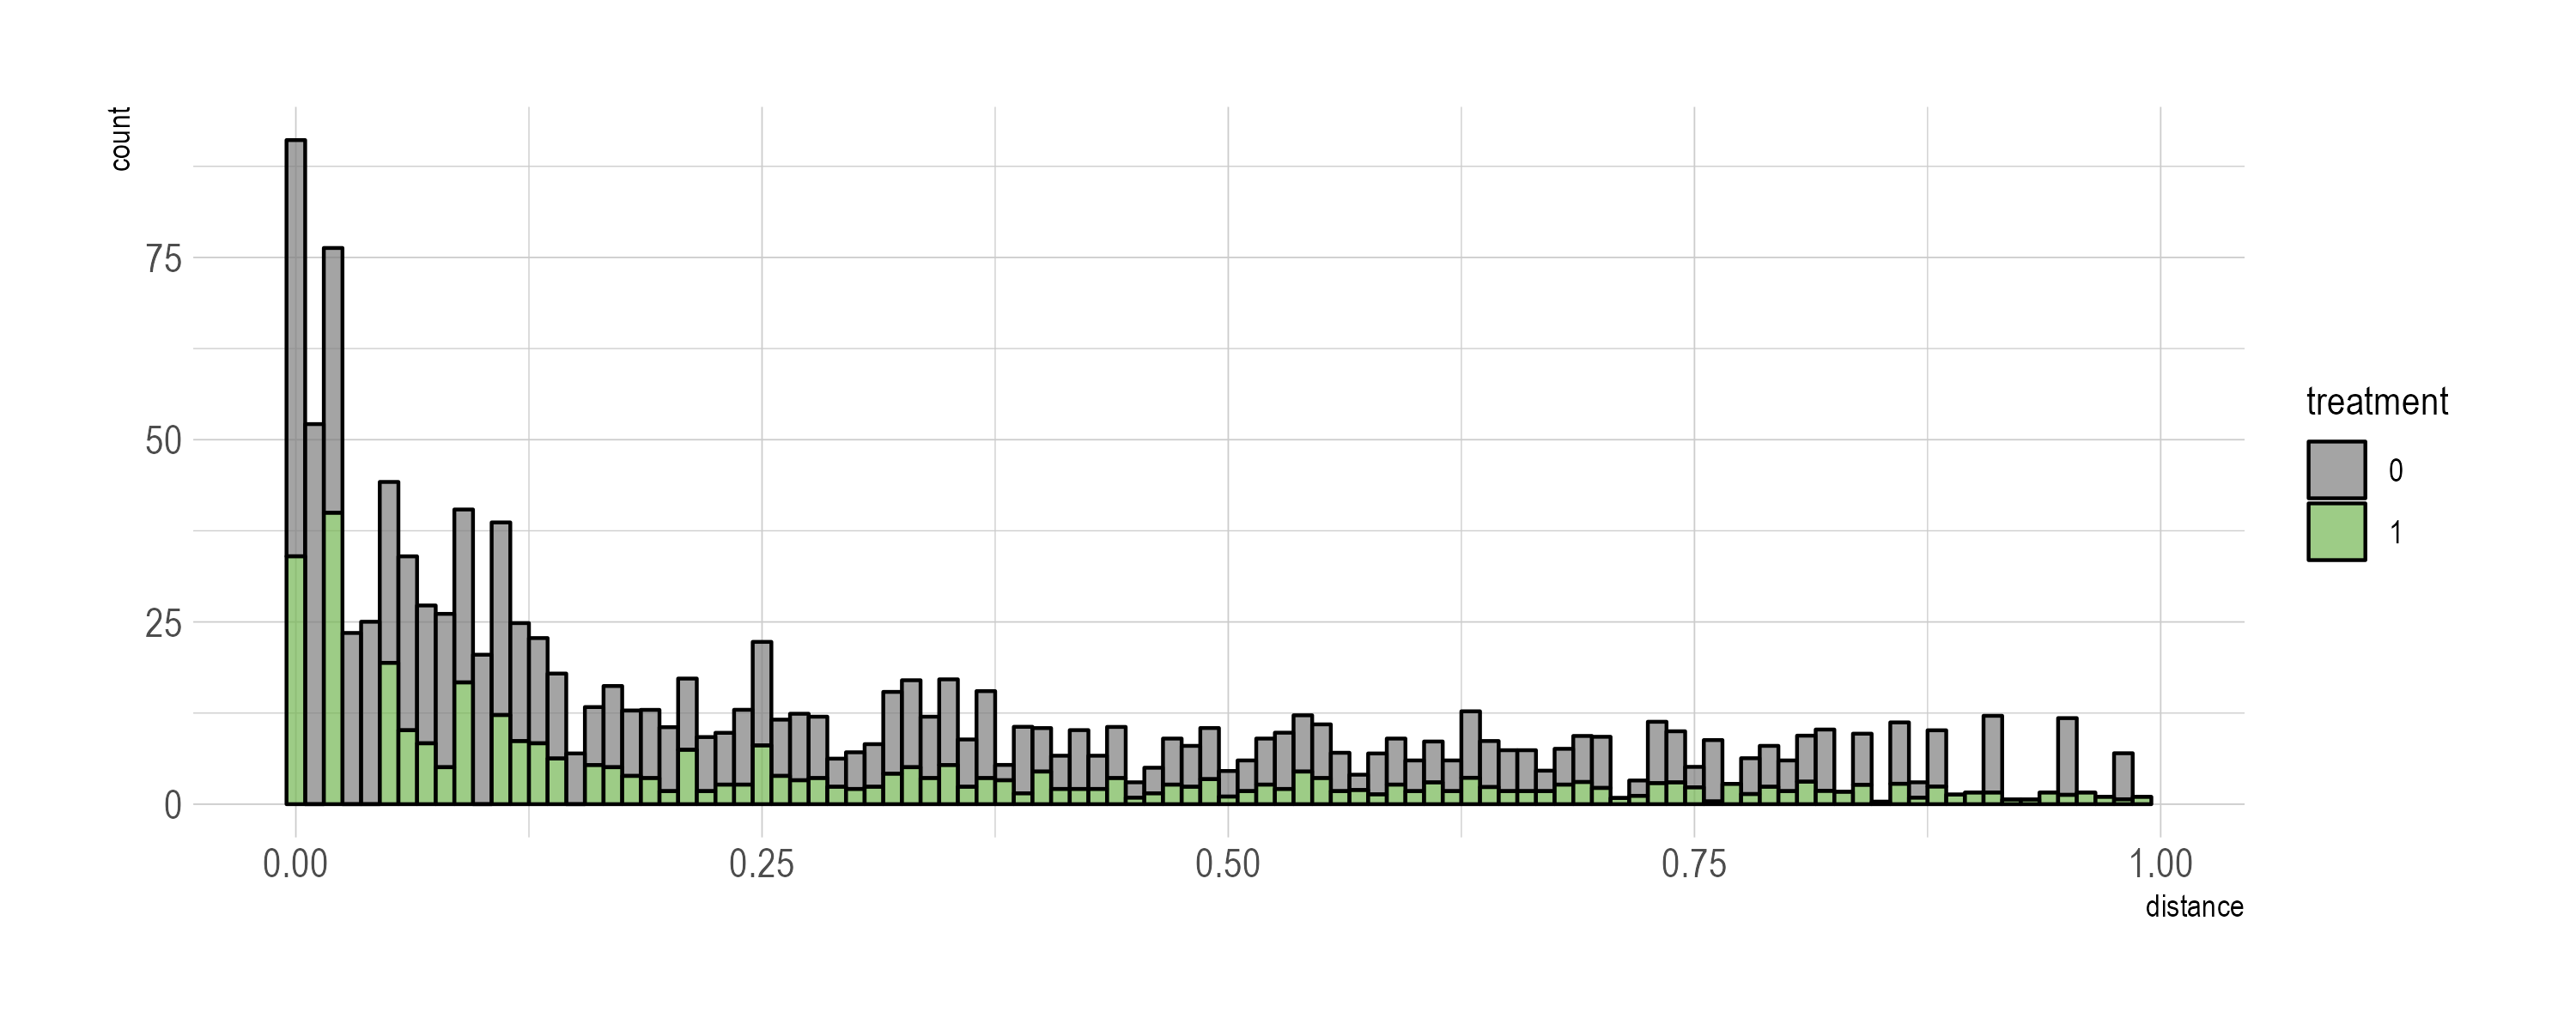
\includegraphics[width=\linewidth]{fig/London/no_title_ss_vegetation_binary_match_result.png}
        \caption*{Vegetation}
    \end{subfigure}%

    \begin{subfigure}{.6\textwidth}
        \centering
        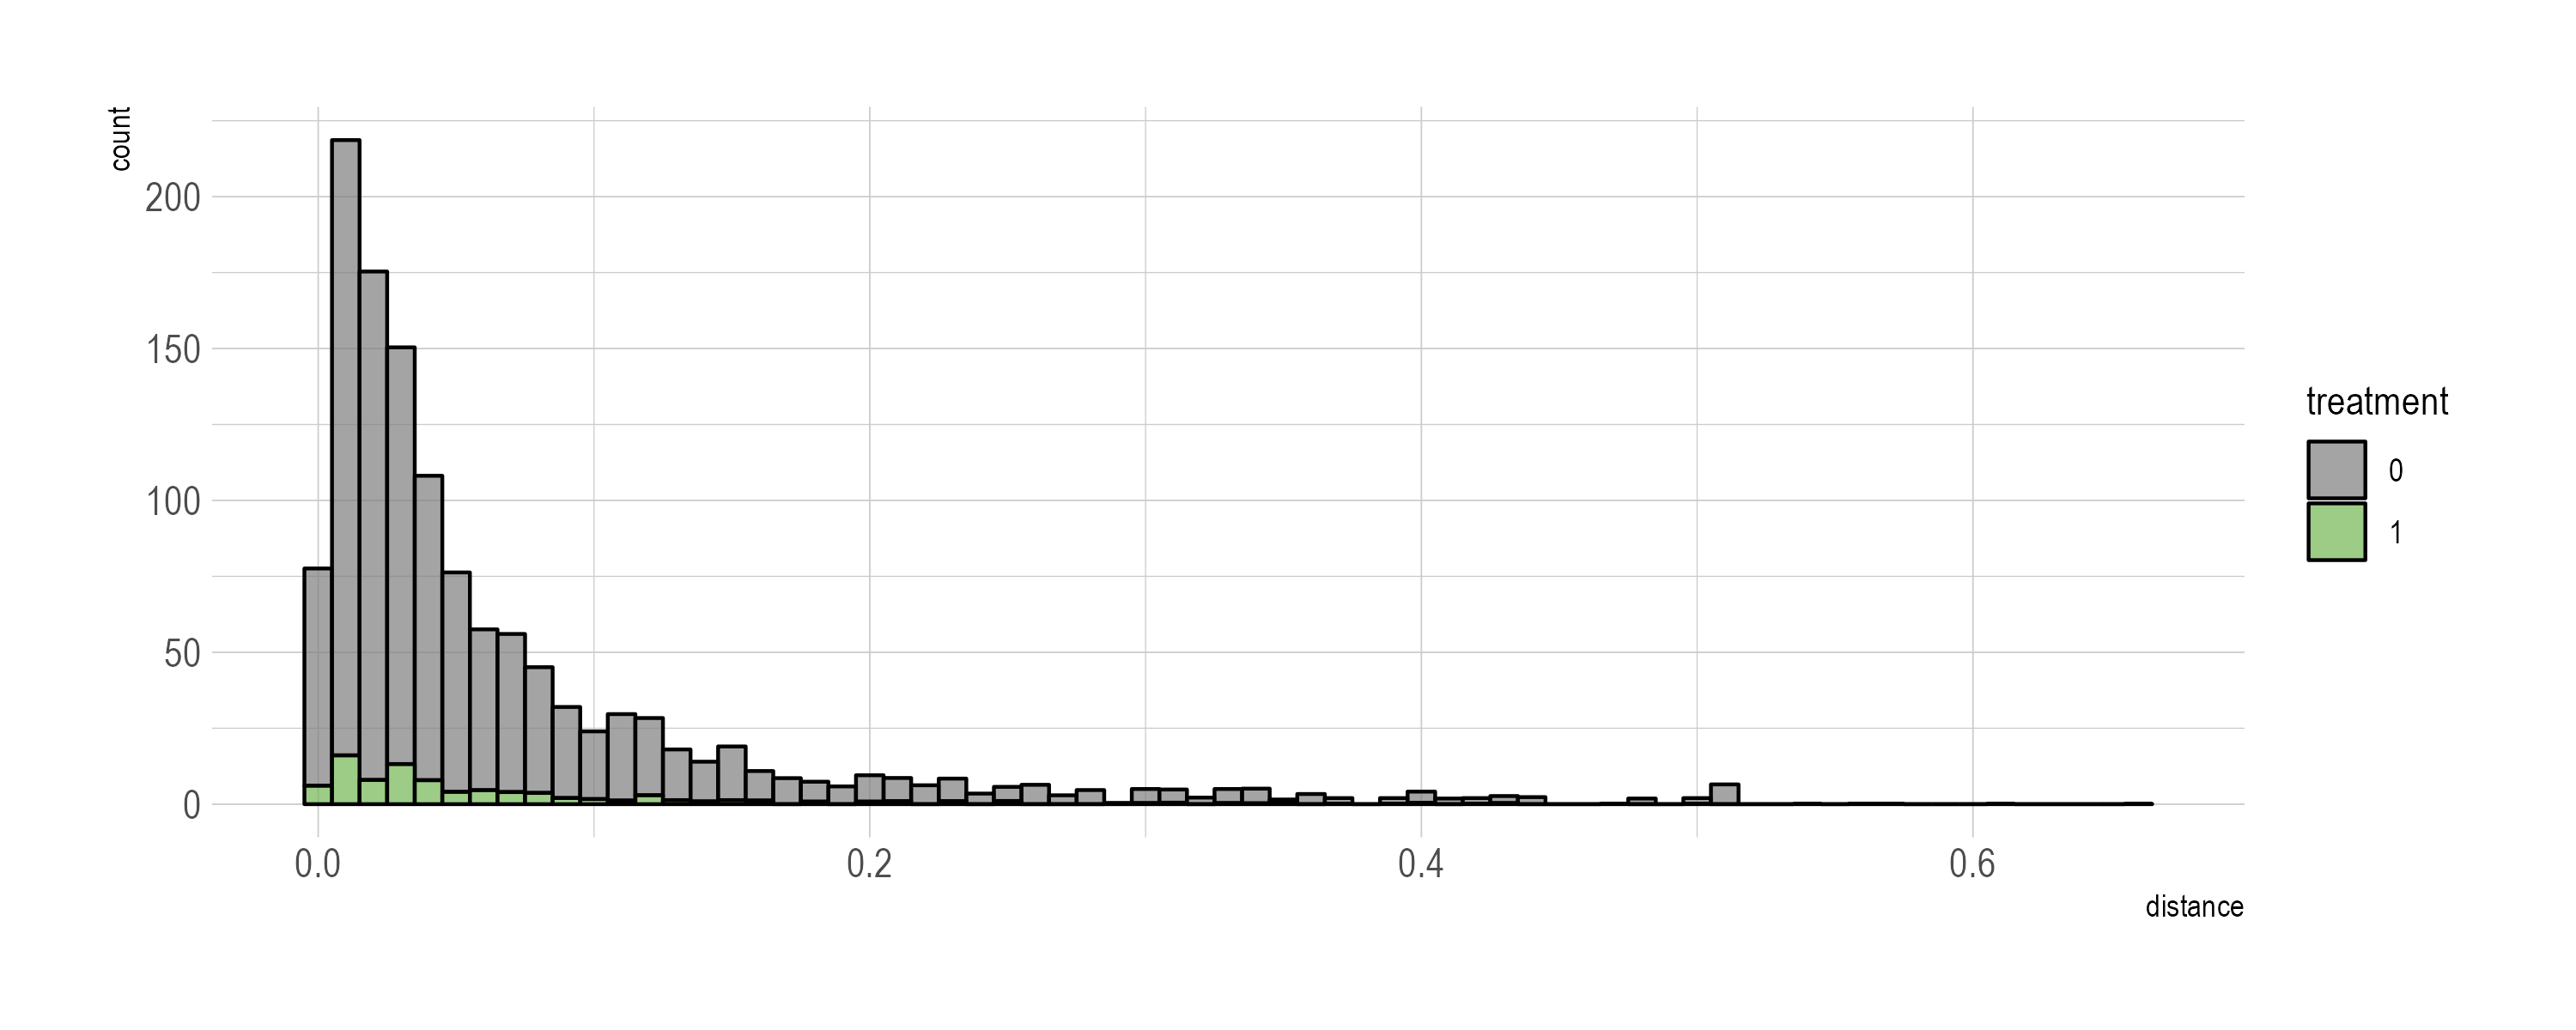
\includegraphics[width=\linewidth]{fig/London/no_title_ss_bike_lane_binary_match_result.png}
        \caption*{Bike Lane}
    \end{subfigure}%

    \begin{subfigure}{.6\textwidth}
        \centering
        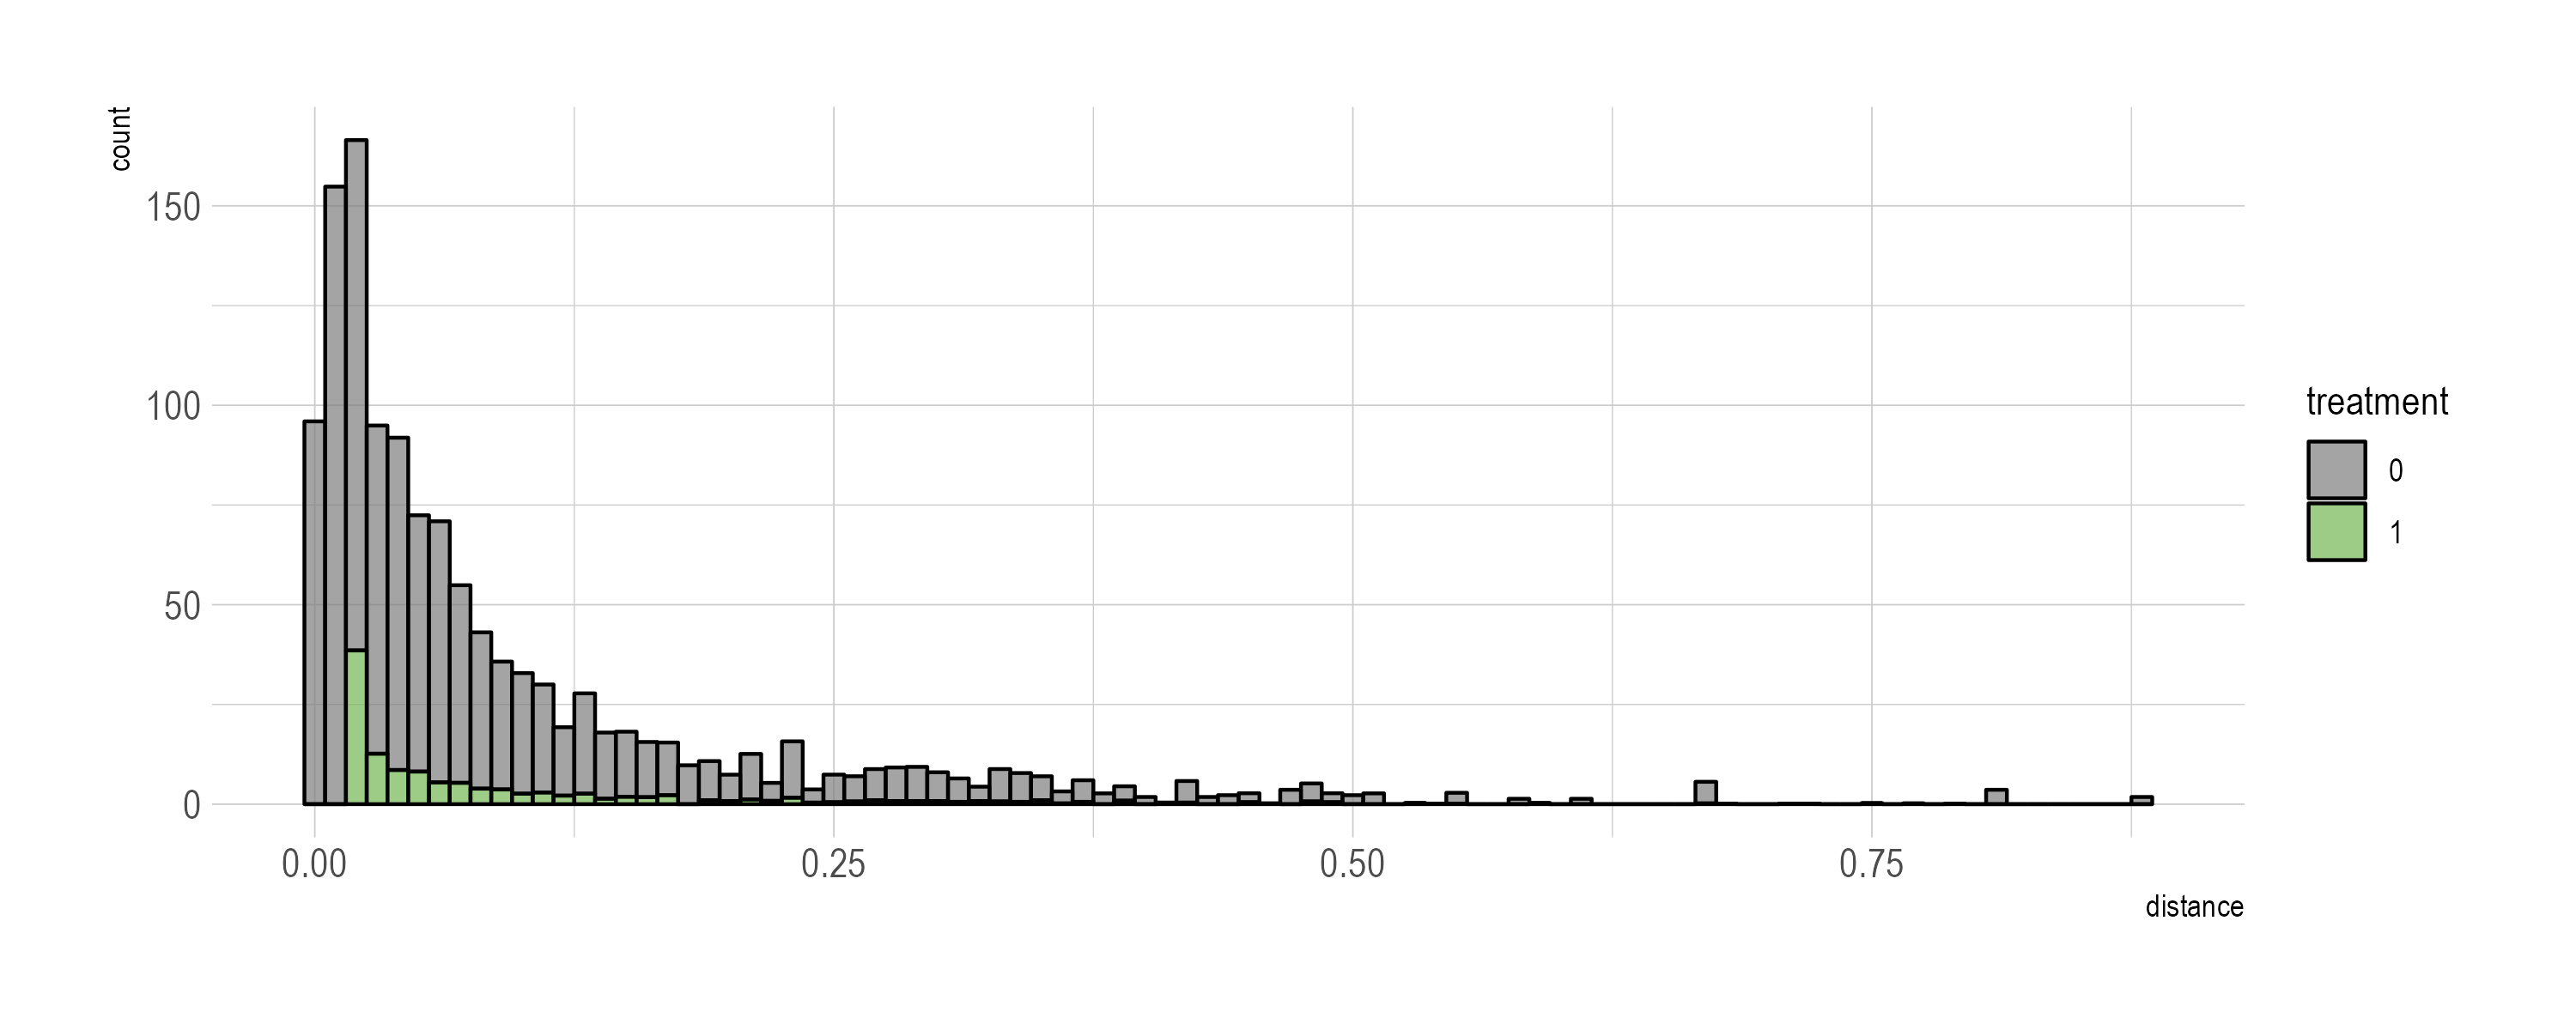
\includegraphics[width=\linewidth]{fig/London/no_title_ss_parking_binary_match_result.png}
        \caption*{Parking}
    \end{subfigure}%

    \begin{subfigure}{.6\textwidth}
        \centering
        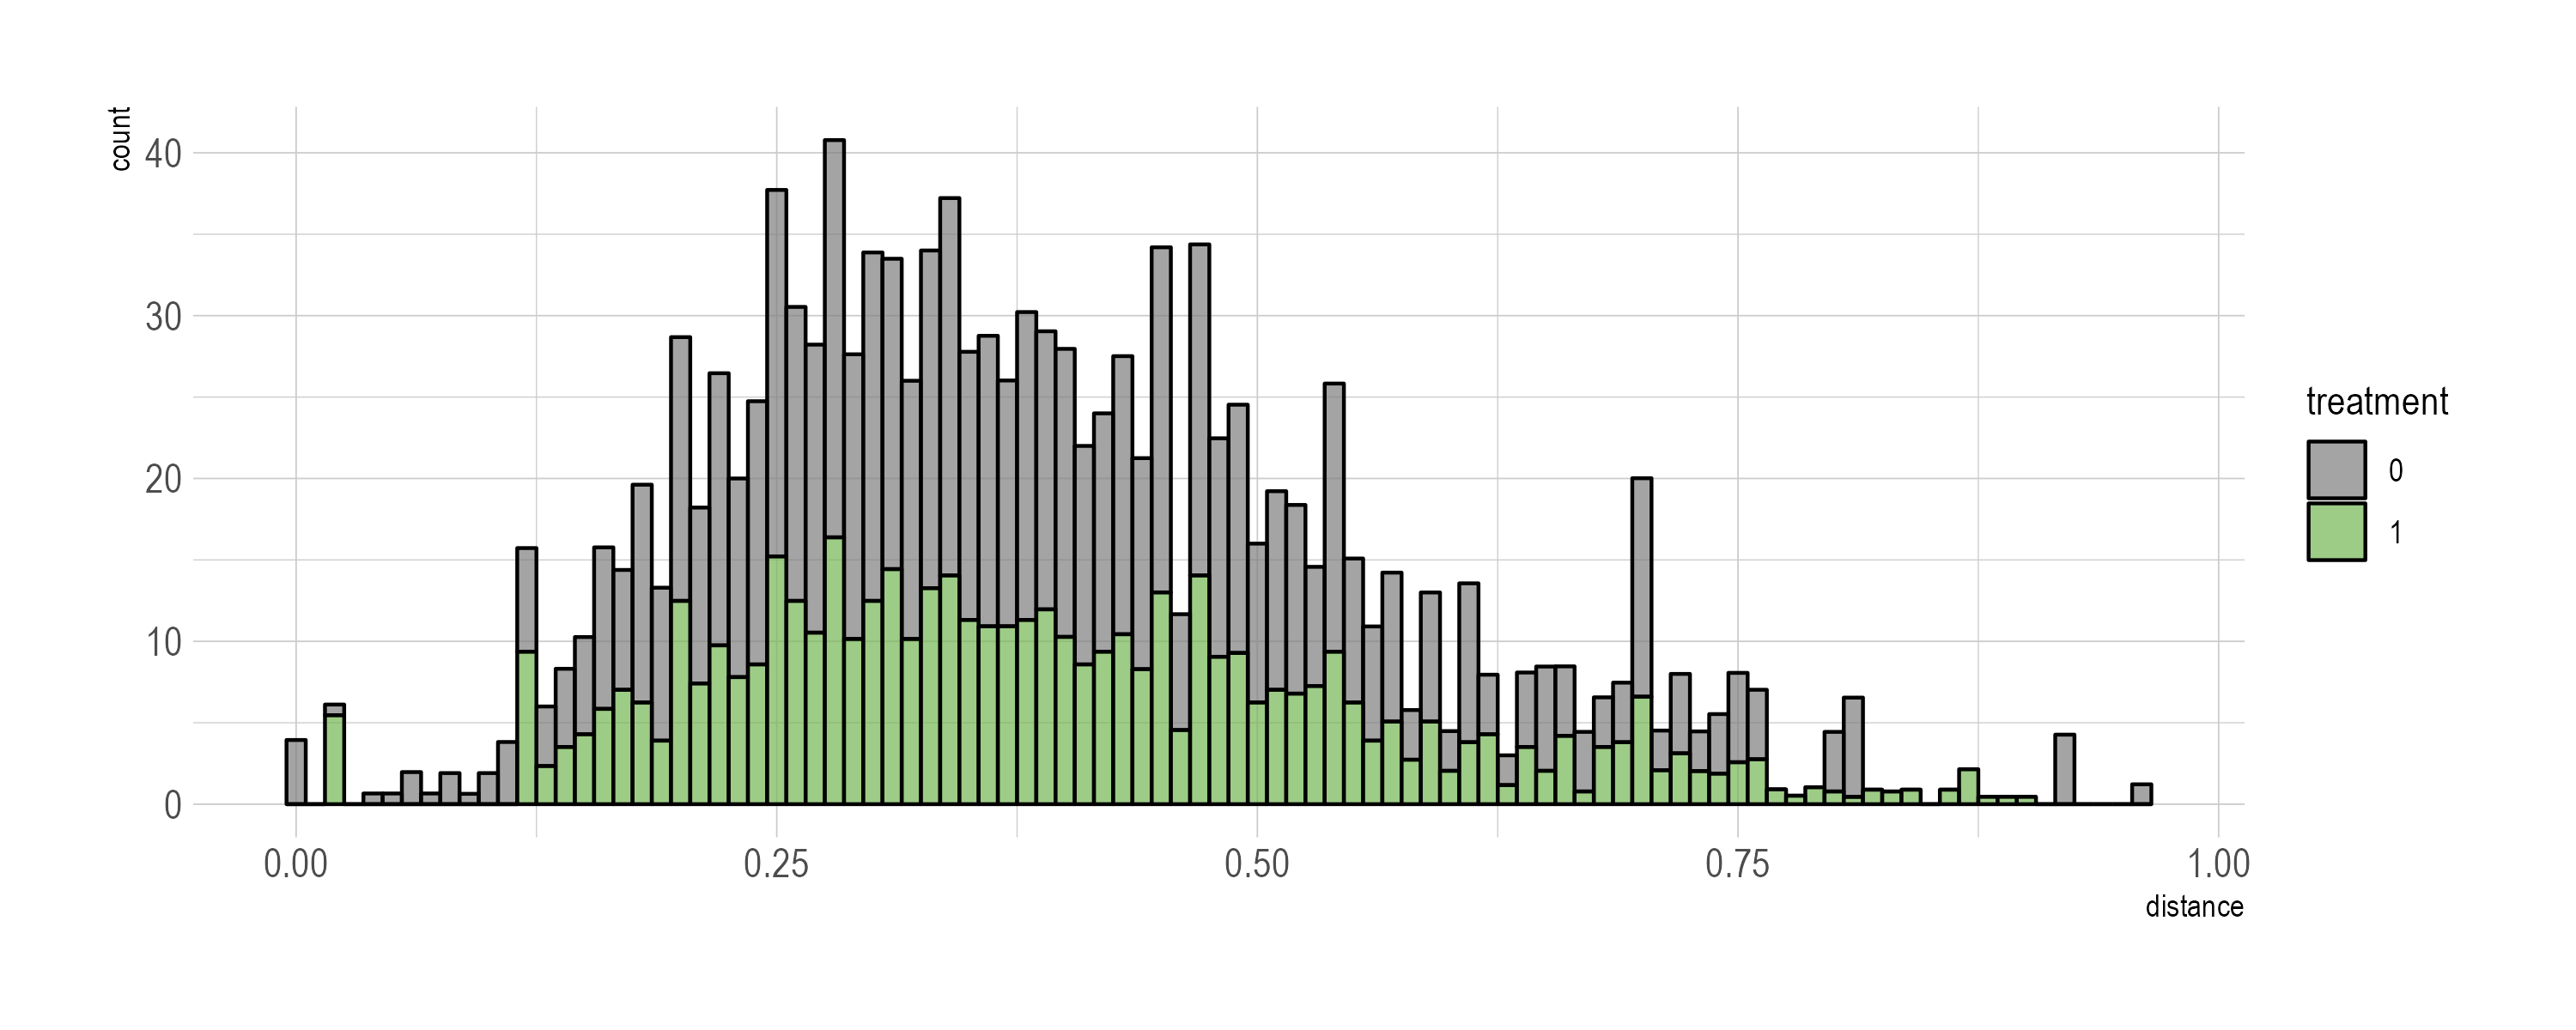
\includegraphics[width=\linewidth]{fig/London/no_title_ss_street_light_binary_match_result.png}
        \caption*{Street Light}
    \end{subfigure}%

    \begin{subfigure}{.6\textwidth}
        \centering
        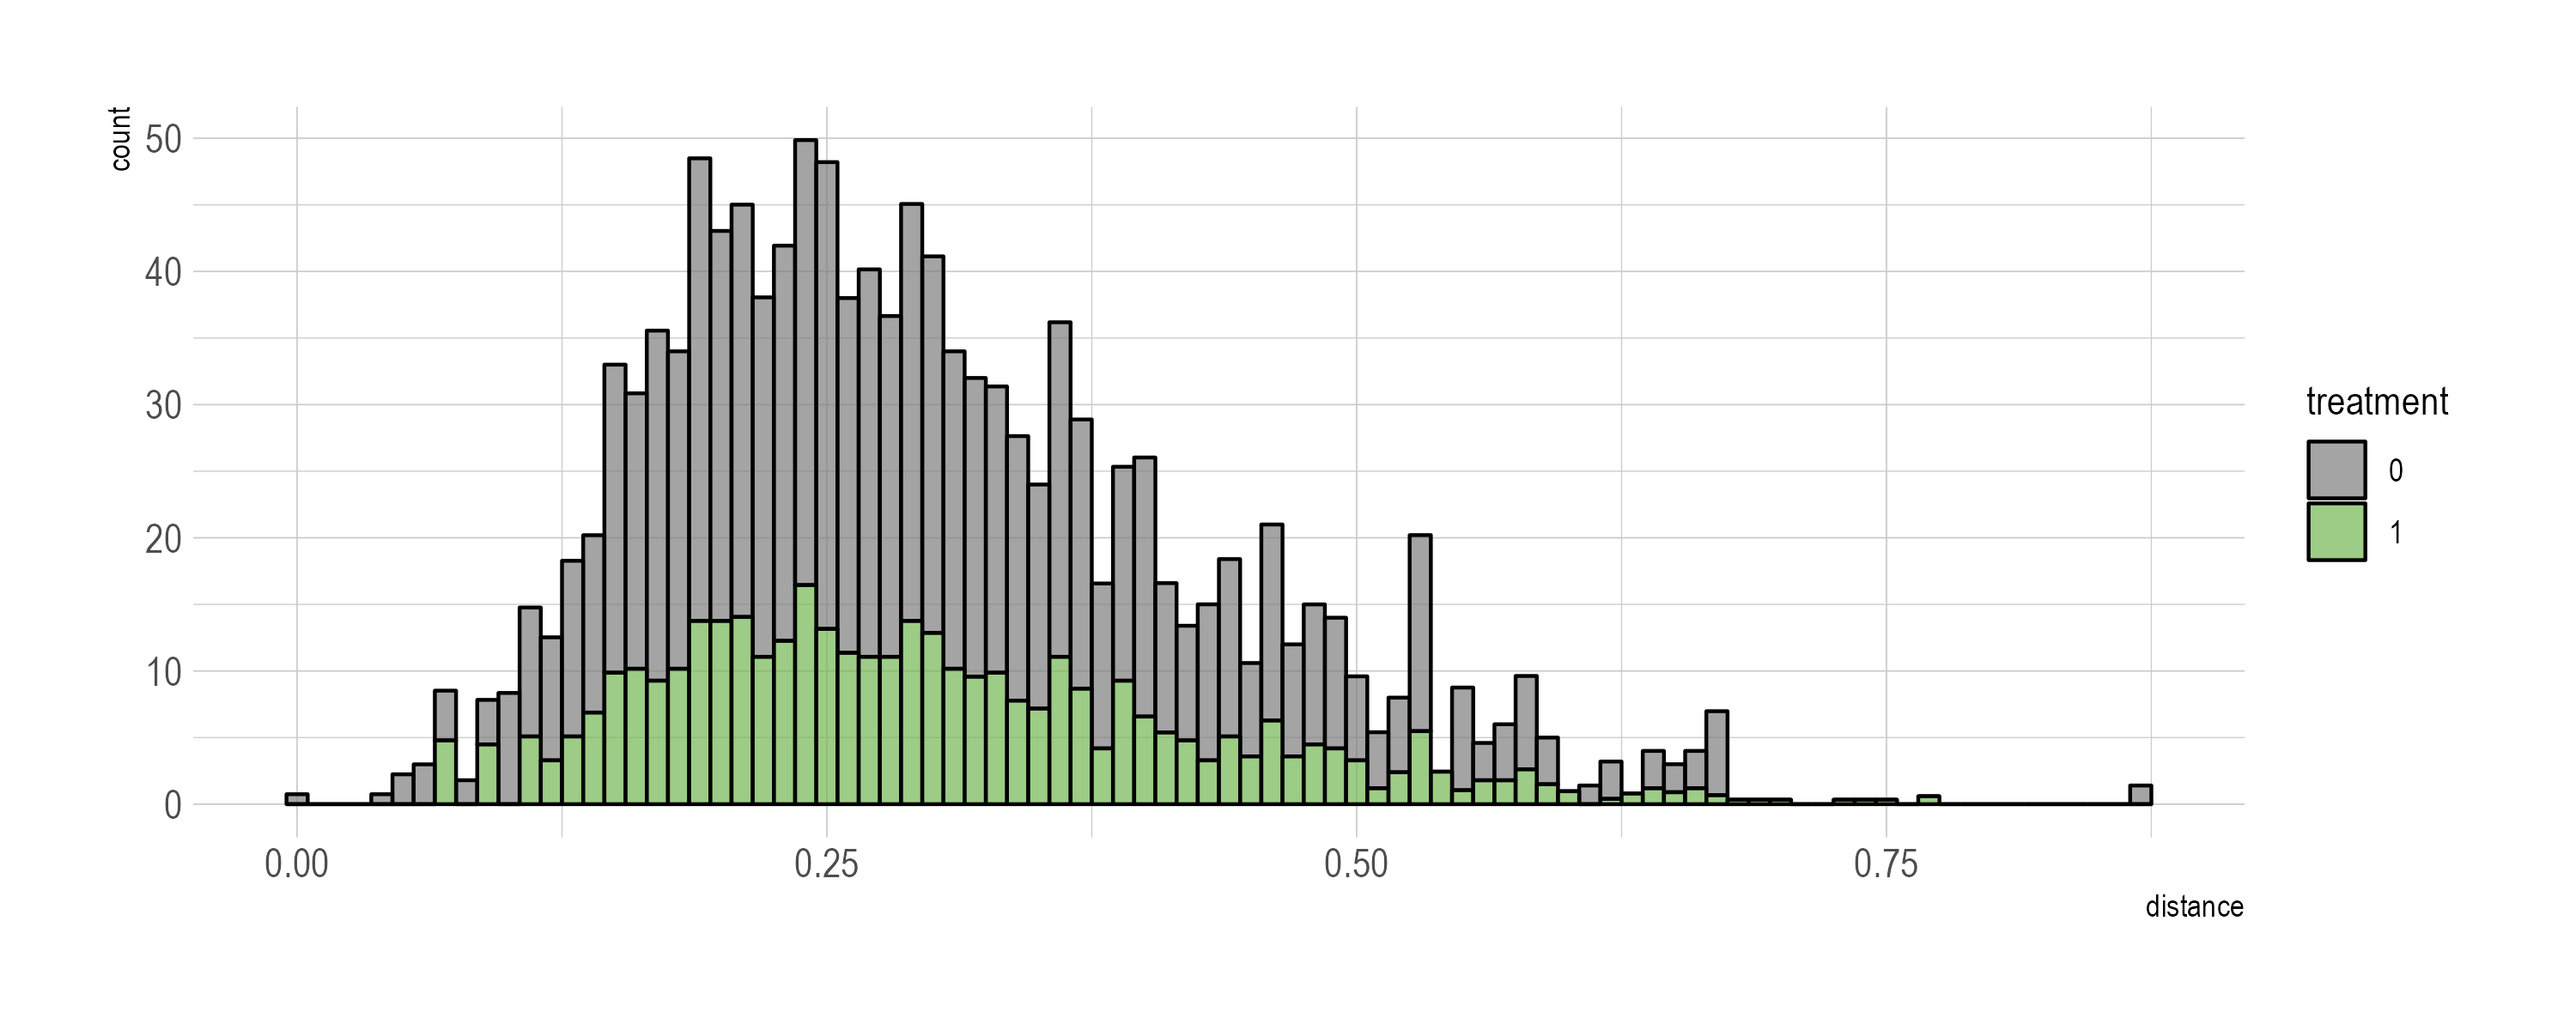
\includegraphics[width=\linewidth]{fig/London/no_title_slope_binary_match_result.png}
        \caption*{Slope}
    \end{subfigure}%

    \caption{Histogram plots illustrate propensity score after matching. The gray parts represent distributions of propensity scores for non-treated units, and the green parts represent treated units. From top to bottom, the plots shows vegetation, bike lane, parking, street light, and slope.}
    \label{result:fig:psm}
\end{figure}

\subsection{Causal Forest}
Finally, the causal forest model was estimated to identify the variable importance and the heterogeneous treatment effects. Covariates for the causal forests models were the same as the ones used for NB-PSM models. \autoref{result:tab:cf} shows the results of the causal forest, which have the same direction and similar statistical significance as the NB-PSM for most of the treatment variables, except for street parking, which changed from significant positive to insignificant negative, and street lights, which changed from insignificant positive to significant positive.
For the variable that changed its significance, direction, or both, further research with different research designs might be needed to draw stronger conclusions in the future.

\begin{table}[!htp]\centering
\caption{CATE of the treatments. The values were rounded to three significant figures.}\label{result:tab:cf}
\scriptsize
\begin{tabular}{lrrrr}\toprule
Variable&Estimate &Standard error \\ \midrule
vegetation& 0.206$^{**}$ & 0.0888 \\
bike lane& 0.334$^{*}$ & 0.176 \\
parking& -0.0234 & 0.113 \\
street light& 0.154$^{*}$ & 0.082 \\
slope& -0.158$^{*}$ & 0.0851 \\
\bottomrule
\textit{Note:}  & \multicolumn{3}{r}{$^{*}$p$<$0.1; $^{**}$p$<$0.05; $^{***}$p$<$0.01} \\
\end{tabular}
\end{table}

Overall, our causal analysis mostly corroborates the findings of previous correlational studies listed in \autoref{lit_review:tab:treatment}, such as the positive impacts of vegetation, bike lanes, and street lights on the number of cyclists observed in Hong Kong, Tokyo, Shenzhen, New Orleans, Washington, D.C., Birmingham, and Seatle \citep{yang_global_2020, nagata_objective_2020, wang_relationship_2020, parker_installation_2011, goodno_evaluation_2013, uttley_road_2020, chen_gps_2018}, and the deterrent effect of slopes as observed in Portland \citep{broach_where_2012}. We identified one interesting finding: the positive effect of street parking on cyclist counts; however, the result was insignificant and negative in the causal forest model. Thus, future research may examine these conflicting results. These findings suggest an overall consistency in the impact of urban design on cycling in different contexts. It is noteworthy that, while our study provides causal evidence, the alignment with prior correlational studies implies that the potential for severe selection bias in these earlier works might not be as significant as presumed, reinforcing the validity of their insights into the relationship between urban design and cycling.

\subsubsection{Variable Importance}
In addition to these estimates, variable importance values were examined in \autoref{result:fig:var_imp}, and these values were calculated based on the number of splits, for which the variables were used to maximize the variance in treatment effects (i.e. heterogeneous treatment effects).

\begin{figure}
    \centering
    \begin{subfigure}{.35\textwidth}
        \centering
        \includegraphics[width=\linewidth]{fig/London/vegetation/no_title_binary_causal_forest_var_imp.png}
        \caption*{Vegetation}
    \end{subfigure}%
    \hfill
    \begin{subfigure}{.35\textwidth}
        \centering
        \includegraphics[width=\linewidth]{fig/London/street_light/no_title_binary_causal_forest_var_imp.png}
        \caption*{Street Light}
    \end{subfigure}

    \begin{subfigure}{.35\textwidth}
        \centering
        \includegraphics[width=\linewidth]{fig/London/bike_lane/no_title_binary_causal_forest_var_imp.png}
        \caption*{Bike Lane}
    \end{subfigure}%
    \hfill
    \begin{subfigure}{.35\textwidth}
        \centering
        \includegraphics[width=\linewidth]{fig/London/slope/no_title_binary_causal_forest_var_imp.png}
        \caption*{Slope}
    \end{subfigure}

    \begin{subfigure}{.35\textwidth}
        \centering
        \includegraphics[width=\linewidth]{fig/London/parking/no_title_binary_causal_forest_var_imp.png}
        \caption*{Parking}
    \end{subfigure}%
    \hfill
    \begin{subfigure}{.35\textwidth}
        % Empty placeholder for alignment
    \end{subfigure}

    \caption{Plots of variable importance. From top to bottom, the left column of the plots shows variable importance computed by causal forest models of vegetation, bike lanes, and parking, and the right column shows street lights and slope.}
    \label{result:fig:var_imp}
\end{figure}

In \autoref{result:fig:var_imp}, the treatment variables have different variables of higher importance, i.e., the variables causing more heterogeneity in the causal effect. 
The top three variables for vegetation in London are related to population density, pixel ratios of human-constructed objects, age groups, and land use for commercial activities, indicating that population and building density introduce heterogeneity in the treatment effect.
Variables with higher importance for bike lanes in London are mostly related to the betweenness of the street network based on POIs, marking on the road, population density, and pixel ratios of human-constructed objects, suggesting that street network, street designs, and crowdedness create heterogeneous effects of such infrastructure.
The heterogeneity in the effect of street parking on cycling count is largely contributed by the number of people detected in SVI, the level of deprivation, and the population density, while that of street lights is mainly contributed by the level of deprivation and land uses.
The heterogeneity in the effect of slope on bicycle counts in London is mostly determined by socioeconomic characteristics, such as age composition and level of deprivation, suggesting that it might affect specific groups of the population.
Overall, from these plots, we observed that visual features extracted from SVI contributed to the heterogeneity in treatment effects, indicating the importance of such features in assessing urban design policies.

\subsubsection{Heterogeneous Treatment Effects}
We obtained several insights from heterogeneous causal effects. 
Firstly, we computed the area under the targeting operator characteristics (AUTOC), which ranges between 0 and 1. A higher AUTOC value (i.e. closer to 1) means that the treatment could be more effectively assigned to increase the outcome, while a lower value (i.e. closer to 0) means that there is little benefit in prioritizing treatment for a specific group and we might as well treat everyone randomly \citep{yadlowsky_evaluating_2021}. 
\autoref{result:tab:autoc} shows AUTOC for each treatment variable. 
AUTOC for vegetation, street parking, and street lights are higher than 0.5, suggesting that providing these treatments in specifically targeted areas can yield more effective results than simply providing them in all the areas equally.

\begin{table}\centering
\caption{This table shows the area under targeting operator characteristics (AUTOC) and 95\% confidence interval (CI).}
\label{result:tab:autoc}
\scriptsize
\begin{tabular}{llrr}\toprule
Variable & AUTOC & 95\% CI \\\midrule
vegetation & 0.55 & 0.15 \\
bike lane & 0.25 & 0.46 \\
parking & 0.54 & 0.27 \\
street light & 0.57 & 0.17 \\
slope & 0.43 & 0.17 \\
\bottomrule
\end{tabular}
\end{table}

\begin{figure}
    \centering

    \begin{subfigure}{.7\textwidth}
        \centering
        \includegraphics[width=\linewidth]{fig/London/vegetation/no_title_hte_by_ranking.png}
        \caption*{Vegetation}
    \end{subfigure}%

    \begin{subfigure}{.7\textwidth}
        \centering
        \includegraphics[width=\linewidth]{fig/London/bike_lane/no_title_hte_by_ranking.png}
        \caption*{Bike Lane}
    \end{subfigure}%

    \begin{subfigure}{.7\textwidth}
        \centering
        \includegraphics[width=\linewidth]{fig/London/parking/no_title_hte_by_ranking.png}
        \caption*{Parking}
    \end{subfigure}

    \begin{subfigure}{.7\textwidth}
        \centering
        \includegraphics[width=\linewidth]{fig/London/street_light/no_title_hte_by_ranking.png}
        \caption*{Street Light}
    \end{subfigure}
    
    \begin{subfigure}{.7\textwidth}
        \centering
        \includegraphics[width=\linewidth]{fig/London/slope/no_title_hte_by_ranking.png}
        \caption*{Slope}
    \end{subfigure}

    \caption{Plots of predicted CATE by ranking. From top to bottom, the plots show variable importance computed by causal forest models of vegetation, bike lanes, parking, street lights, and slope. The purple dots represent the estimated CATE for the observations, and the gray areas represent the 95\% confidence intervals.}
    \label{result:fig:rank_cate}
\end{figure}



\begin{figure}
    \centering
    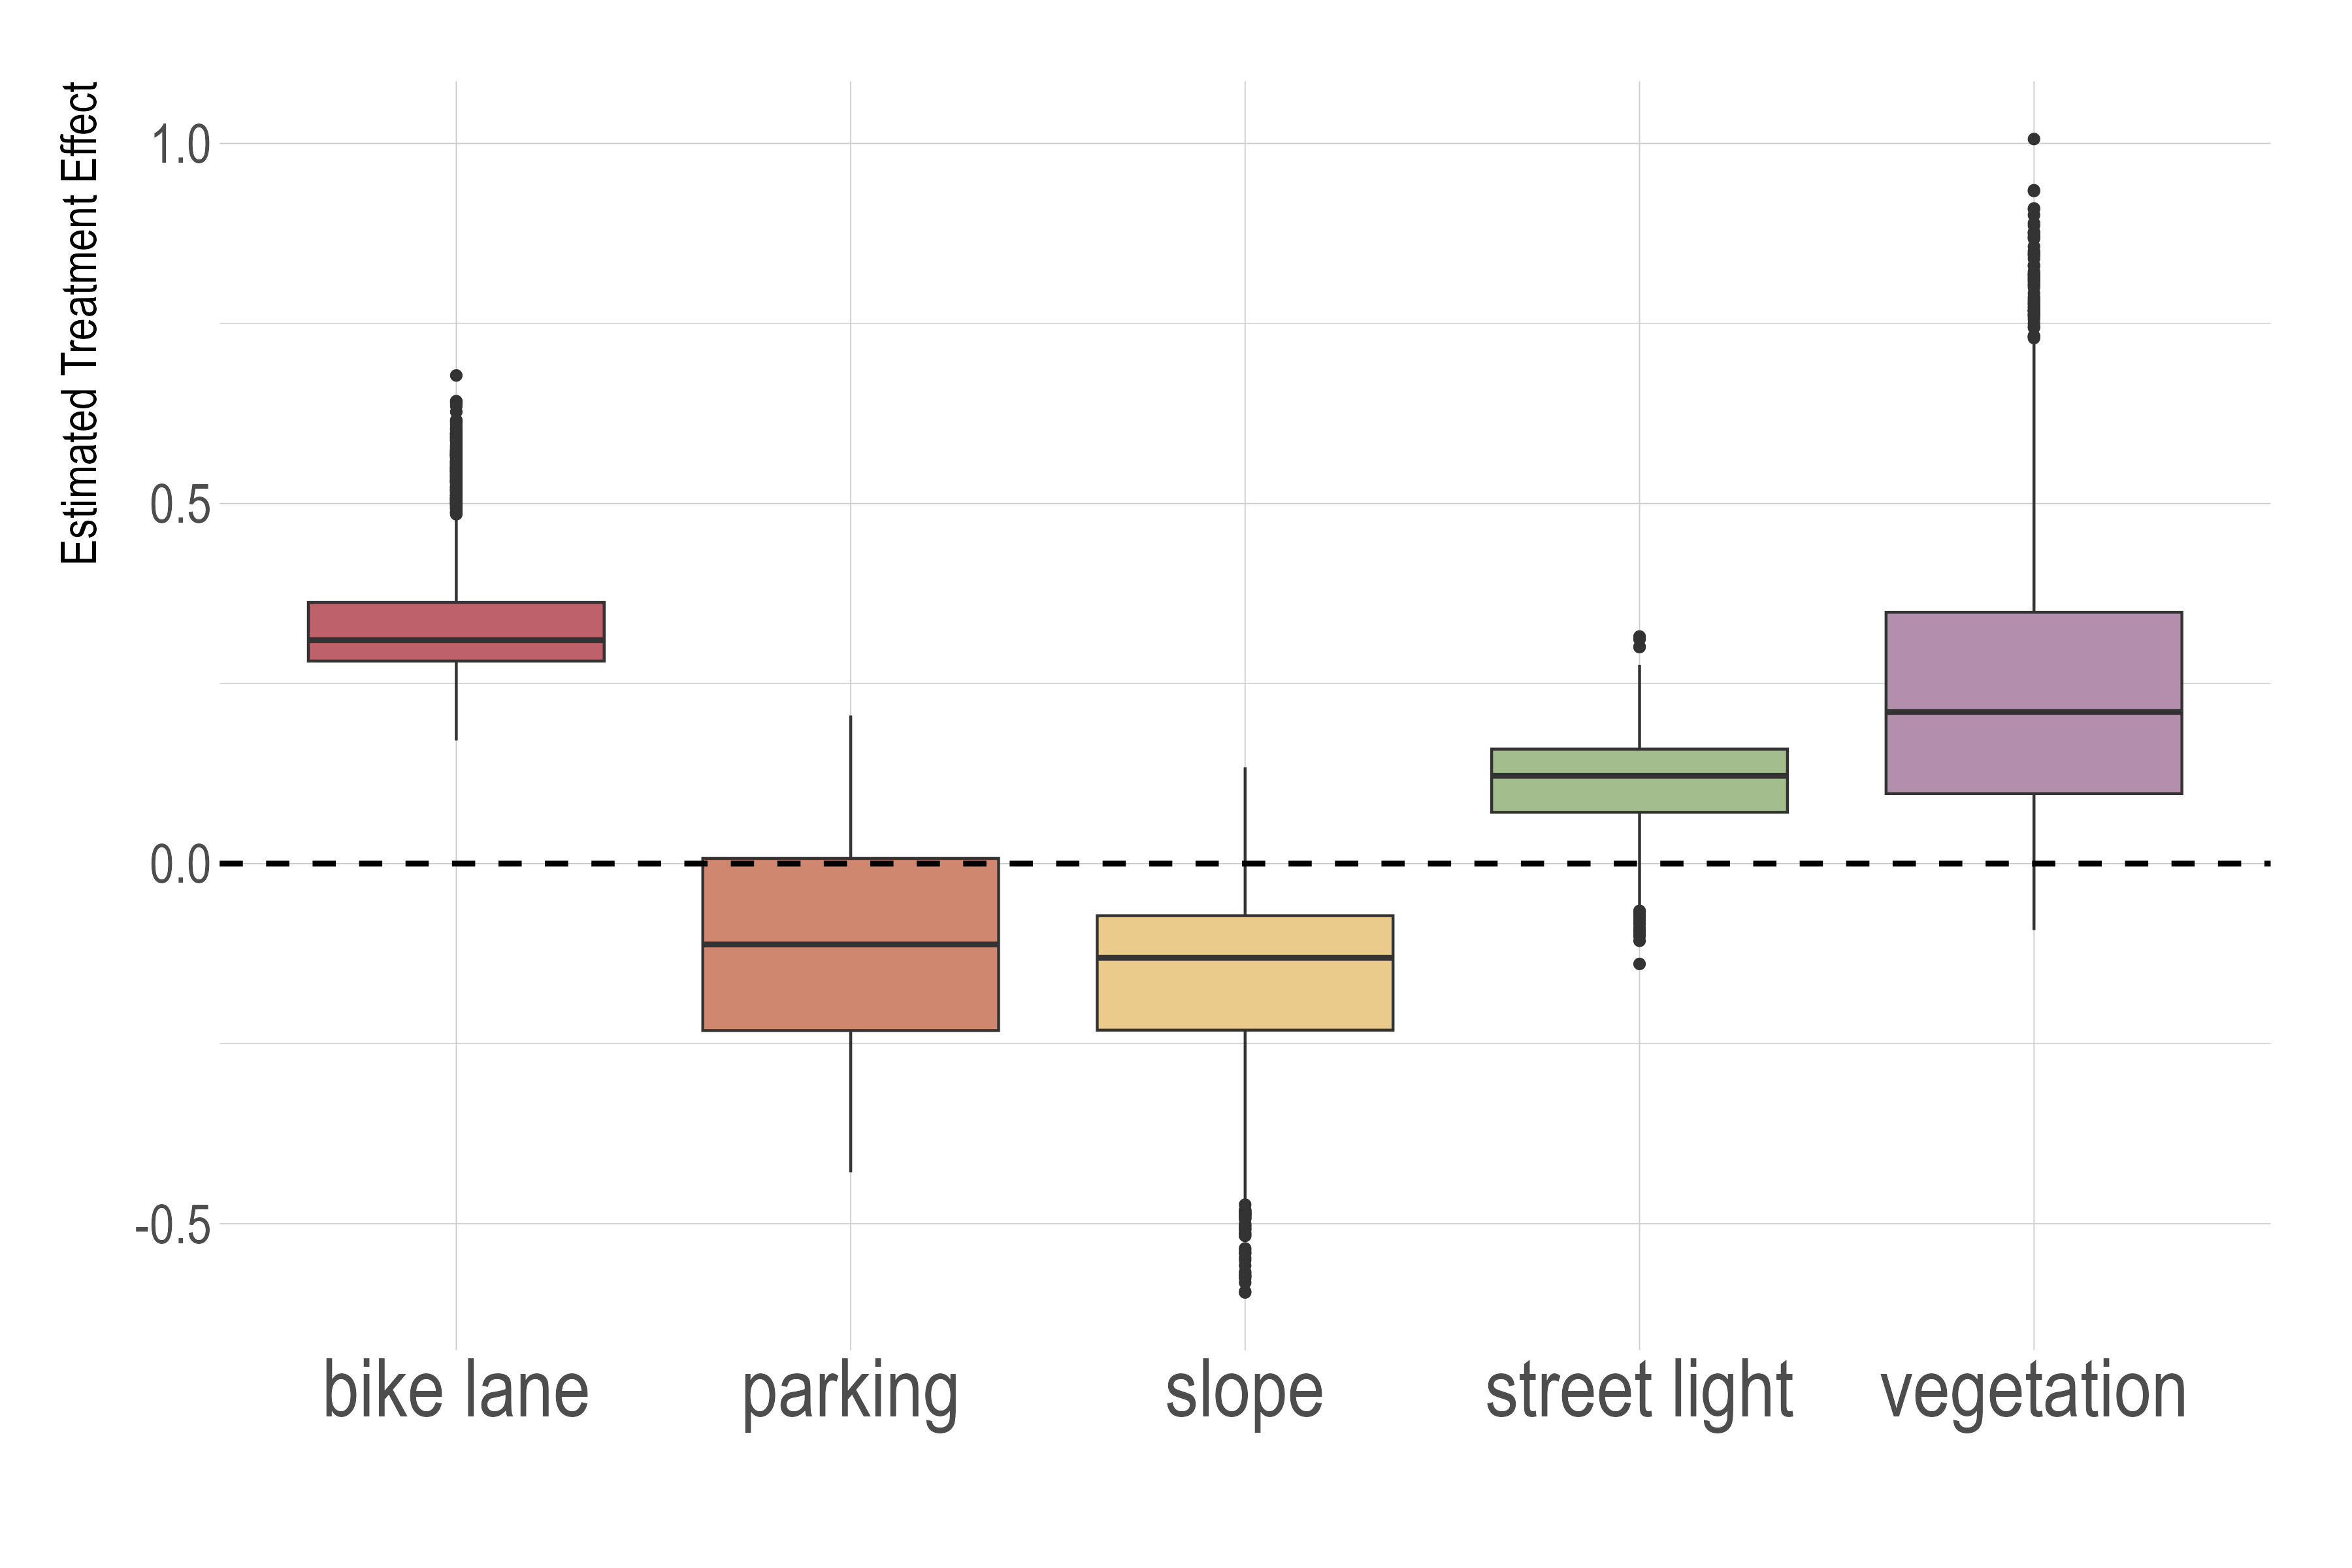
\includegraphics[width=\textwidth]{fig/London/combined_hte_boxplot_no_title.png}
    \caption{This figure displays box plots of the estimated treatment effects for the five treatments by using all the observations. The dashed line at zero represents no effect.}
    \label{result:fig:cate_boxplots}
\end{figure}


To further investigate such heterogeneous effects, we rank CATE values for each unit. The results are visualized in \autoref{result:fig:rank_cate}, where the purple dots indicate estimates of treatment effects, and the gray areas represent the 95\% confidence interval. The existence of heterogeneous effects for all treatment indicators is evident in the figure. Among notable effects, while most observations have positive treatment effects of vegetation, bike lanes, and street lights, the treatment effect is negative for most observations for slope. Overall, the directions of the treatment effects are also consistent with the findings in the earlier-discussed main model.
In addition, plots for those with higher AUTOC have sharper upward trends on the right end and sharper downward trends on the left end than those with lower AUTOC, confirming that policymakers can create larger treatment effects by prioritizing units with higher ranks. 

\autoref{result:fig:cate_boxplots} illustrates the estimated treatment effects across the treatment variables by using the same CATE values from \autoref{result:fig:rank_cate}. The results reveal the same patterns as \autoref{result:fig:rank_cate}, with bike lanes and vegetation showing predominantly positive effects, street lights demonstrating mixed but generally positive outcomes, and parking and slope exhibiting largely negative influences. Based on these findings, policymakers and urban planners need to be aware of the varying effects of treatments, especially when implementing interventions that show positive effects on average but have some observations with negative effects as it is likely that treatment effects differ in various contexts.

To further investigate how treatment effects change across different contexts, we divided datasets into three groups based on each covariate's percentiles (i.e., 0\% < covariate's value <= 33\%, 33\% < covariate's value <= 66\%, and 66\% < covariate's value) and examined non-linear treatment effects in three subgroups in a more data-driven and nuanced way.
\autoref{result:fig:rank_cate_covariates} shows four covariates with the highest differences among the three groups. The figures include error bars representing 90\% confidence intervals; thus, the treatment effect is statistically different at a significance level of 0.1 or smaller if at least two of the error bars of the ``0-33\%", ``33-66\%", and ``66-100\%" groups do not overlap. 

For vegetation, four covariates have statistically different treatment effects between the three subgroups. The treatment effects of vegetation on bicycle counts are higher when the population of the age group between 0 and 19 is in 33-66\% than in 66-100\%, IMD score is in 0-66\% than 66-100\%, the number of persons detected in SVI is in 0-33\% than in 66-100\%, and population density is in 0-33\% than in 66-100\%. This might indicate that a moderate proportion of young residents may be more inclined to cycle in greener areas, but the effect lowers in areas with very high or low youth populations. Similarly, areas with an IMD score in the 0-66\% range see greater benefits from vegetation, suggesting that while less deprived areas already conducive to cycling gain from added greenery, the most deprived areas might not capitalize on these benefits due to deeper socioeconomic barriers.
The treatment effects are also more pronounced in areas with fewer persons detected in SVI (0-33\%), highlighting a preference for cycling in less crowded, green environments. However, in densely populated areas, congestion could dilute the positive impact of vegetation. Additionally, lower population density areas (0-33\%) experience a stronger influence of vegetation on cycling activities, reflecting the appeal of spacious and green settings for cycling. Yet, this effect is moderated in both very low and high-density areas, where infrastructure and urban congestion respectively might limit the utility of green spaces for encouraging cycling.

For bike lanes, the effectiveness is markedly higher on the streets with high (66-100\%) and low (0-33\%) traffic speeds than on those with moderate traffic speeds (33-66\%) and the most densely populated areas (66-100\%) compared to moderately dense areas (33-66\%). This suggests that bike lanes are particularly beneficial along high-speed roads because bike lanes likely provide a significant perceived safety benefit, encouraging more cyclists, as well as along low-speed roads because the lanes may enhance cyclists' visibility and legitimacy, improving interactions with motorists. The negative effect observed on moderate-speed roads is intriguing and warrants further investigation. It could potentially be explained by a combination of factors: cyclists might feel less need for dedicated infrastructure on these roads, leading to reduced usage of the bike lanes; the lanes might inadvertently create a false sense of security, leading to riskier behavior; or the implementation of bike lanes on moderate-speed roads might result in traffic flow changes that negatively impact cycling conditions. Additionally, the negative effect could be due to unintended consequences, such as increased conflict points at intersections or driveways, which may be more numerous on moderate-speed roads. 
In addition, bike lanes can promote cycling in urban cores where the demand for efficient transportation alternatives is greatest, possibly due to the higher concentration of cyclists and the potential to reduce vehicular traffic. 

The treatment effect of street parking is worse in areas with a percentage of age group between 0 and 19 in 0-33\% than in 66-100\% and the level of deprivation in 33-66\% than in 66-100\%. This might indicate that street parking, by occupying space that could otherwise support cycling infrastructure, disproportionately affects areas where cycling might serve as a critical mobility option for those not served by the youth demographic or facing moderate socioeconomic challenges. The analysis did not reveal statistically significant variations in the treatment effects of street lights on cycling, suggesting that the presence or absence of street lighting may not distinctly influence cycling patterns across different demographics or levels of urban density.

Regarding slope, its deterrent effect on cycling becomes significantly stronger in regions with a higher proportion of older residents (age group 40-59 in the 66-100\% range and age group 20-39 in the 0-33\% range) compared to a moderate proportion (age group 40-59 in the 33-66\% range and age group 20-39 in the 33-66\% range). This finding underscores the physical challenges and safety concerns that steeper terrains pose to older cyclists, highlighting the need for targeted interventions in hillier areas to maintain or enhance cycling accessibility for aging populations. Moreover, slope had a positive effect on cyclist counts in the most deprived areas (66-100\%) while it had a significantly lower and negative effect on cyclist counts in the least deprived areas (0-33\%), potentially indicating that wealthier populations are affected by unfriendly cycling environment more easily because the financial barrier for them to switch to alternative modes of transportation (e.g., private vehicles) is lower. Lastly, slope also had a positive effect in non-residential areas (0-33\%) while it had a negative effect in the residential areas (66-100\%), suggesting that people might be willing to cycle on hilly terrains for leisure in non-residential areas. 

 For urban planners, landscape architects, and policymakers, these findings emphasize the importance of considering the local context and physical characteristics of an area when designing interventions aimed at increasing cyclist count. By prioritizing enhancements in areas where they can have the most substantial effect, it is possible to create urban environments that are more conducive to cycling, thereby promoting healthier and more active communities.

\begin{figure}
    \centering

    \begin{subfigure}{.42\textwidth}
        \centering
        \includegraphics[width=\linewidth]{fig/London/vegetation/no_title_hte_by_covariate.png}
        \caption*{Vegetation}
    \end{subfigure}%
    \hfill
    \begin{subfigure}{.42\textwidth}
        \centering
        \includegraphics[width=\linewidth]{fig/London/street_light/no_title_hte_by_covariate.png}
        \caption*{Street Light}
    \end{subfigure}

    \begin{subfigure}{.42\textwidth}
        \centering
        \includegraphics[width=\linewidth]{fig/London/bike_lane/no_title_hte_by_covariate.png}
        \caption*{Bike Lane}
    \end{subfigure}%
    \hfill
    \begin{subfigure}{.42\textwidth}
        \centering
        \includegraphics[width=\linewidth]{fig/London/slope/no_title_hte_by_covariate.png}
        \caption*{Slope}
    \end{subfigure}

    \begin{subfigure}{.42\textwidth}
        \centering
        \includegraphics[width=\linewidth]{fig/London/parking/no_title_hte_by_covariate.png}
        \caption*{Parking}
    \end{subfigure}
    \hfill
    \begin{subfigure}{.4\textwidth}
        % Empty placeholder for alignment
    \end{subfigure}

    \caption{Plots of CATE by subgroups of covariates. From top to bottom, the left column of the plots shows CATE by subgroups of covariates (i.e., heterogeneous treatment effects) for vegetation, bike lanes, and parking, and the right column shows street lights and slope. The purple lines represent the 0-33\% group of covariates, the yellow lines represent the 33-66\% group, and the green lines represent the 66-100\% group. The center points are the estimated CATE, and the lines are the 90\% confidence intervals.}
    \label{result:fig:rank_cate_covariates}
\end{figure}
    
% Lastly, a non-causal method was explored to examine how policy implications would change, and the result of a zero-inflated negative binomial model is shown in \autoref{result:tab:zinb}.
% Vegetation had a significantly negative estimate, which is a different result from both the two causal methods and the previous studies that reported a significant positive correlation between greenery and cycling activities \citep{yang_global_2020, nagata_objective_2020, wang_relationship_2020}, while slope had significant correlations in the same direction as the causal methods. 
% The difference in vegetation from the previous study can be explained by the scale and context of the studies. 
% All the previous studies have smaller study areas (e.g., Hong Kong, areas around metro stations in Shenzhen, and a ward in Tokyo) than the Greater London area used in our study, which might have provided more similar distribution of covariates (i.e. less selection bias) than our study area that includes the central business district and suburbs \citep{yang_global_2020, nagata_objective_2020, wang_relationship_2020}. 
% The purposes of cycling differ based on the contexts; thus, a more heterogeneous environment in London might have led to the opposite result from the previous study.
% The difference from the causal methods can be then explained by selection bias. 
% \autoref{result:fig:map_grid} shows that a higher number of cyclist counts are concentrated in the central area, while more greenery is distributed in the peripheral area; therefore, a simple regression model without matching observations with similar covariates possibly led to a biased estimate. 
% These findings indicate the value of this study for policymakers --- finding the unbiased treatment effects with heterogeneous large-scale data, and simplistic analysis could have led to a wrong policy implication.

% % Table created by stargazer v.5.2.3 by Marek Hlavac, Social Policy Institute. E-mail: marek.hlavac at gmail.com
% % Date and time: Tue, Dec 06, 2022 - 11:28:14
% \begin{table}[!htbp] \centering 
%   \caption{The result of a zero-inflated negative binomial model without removing selection bias.} 
%   \label{result:tab:zinb} 
% \scriptsize 
% \begin{tabular}{@{\extracolsep{1pt}}lc} 
% \\[-1.8ex]\hline 
% \hline \\[-1.8ex] 
%  & \multicolumn{1}{c}{\textit{Dependent variable:}} \\ 
% \cline{2-2} 
% \\[-1.8ex] & pedal\_cycles \\ 
% \hline \\[-1.8ex] 
%  ss\_vegetation & $-$0.626$^{***}$ (0.002) \\ 
%   ss\_sidewalk & 1.073$^{***}$ (0.007) \\ 
%   IMD\_score & 0.007$^{***}$ (0.00002) \\ 
%   housing\_price\_log & 0.341$^{***}$ (0.001) \\ 
%   poi\_log & 0.463$^{***}$ (0.0002) \\ 
%   slope & $-$0.181$^{***}$ (0.0003) \\ 
%   pop\_den\_log & 0.067$^{***}$ (0.0004) \\ 
%   lu\_residential & $-$0.018$^{***}$ (0.00005) \\ 
%   Constant & 0.474$^{***}$ (0.008) \\ 
%  \hline \\[-1.8ex] 
% Observations & 23,265 \\ 
% Log Likelihood & $-$8,248,416.000 \\ 
% \hline 
% \hline \\[-1.8ex] 
% \textit{Note:}  & \multicolumn{1}{r}{$^{*}$p$<$0.1; $^{**}$p$<$0.05; $^{***}$p$<$0.01} \\ 
% \end{tabular} 
% \end{table} 

% \begin{figure}
%     \centering
%     \includegraphics[width=\textwidth]{fig/map_grid.png}
%     \label{result:fig:map_grid}
%     \caption{A map of cyclist counts and greenery in London.}
% \end{figure}
\clearpage
\subsection{Limitations}
Despite its novelty, this paper has some limitations, which open avenues for future research.
The first limitation is related to the quality of the count data on cycling activities and the SVI data.
The count data have only been collected by Transport for London once a year and do not have information on the time of the day. 
Therefore, our study is susceptible to biases due to spatially varying weather conditions and trends of cyclists' activities across different count stations even after the year-month fixed effects. 

SVI might have introduced a bias as well.
SVI collected by Google are usually taken by cameras mounted on top of vehicles, so they are taken from the middle of roads, not from the road shoulders or sidewalks, where people cycle.
Further, off-road venues where there may also be cycling traffic are not always covered by street-level imagery~\citep{2023_cities_pos}.
When analyzing street features to understand cyclists' experiences, such a discrepancy could have decreased the accuracy of the analysis.
We also used pixel ratios of segmented SVI as proxies for the presence and visual impact of elements, such as vegetation and street furniture. While this method allows for standardized comparisons across different scenes, it does not directly measure the physical dimensions of these features, highlighting the need to develop more precise methods for evaluating urban design elements and their influence on cycling.
Future research can address these issues by collecting more granular data through GPS trackers and obtaining SVI from the perspectives of cyclists with deep learning techniques such as generative adversarial networks, or taking advantage of crowdsourced SVI services such as Mapillary and KartaView that increasingly include such perspectives~\citep{ito_translating_2024, hou_global_2024, 2023_jag_svi_sensitivity}.

Another limitation is the nature of this paper ––– an observational study.
Despite the effort to match treated and untreated units through PSM and causal forests, some unobserved confounding is inevitable compared to more controlled research settings, such as randomized controlled trials. Thus, future research can validate the results of this study by conducting a smaller-scale experiment in a more controlled setting and analyzing cyclists' perceptions of different types of built environments by recording their brain data through an electroencephalogram (EEG) device. 

Recognizing the limitations of data availability, our study adopts an aggregated-level approach due to the practical challenges of collecting individual-level data across an entire city. This strategy allows for the examination of overall trends in cycling, providing insights into the collective impact of urban design features on cycling activities. However, we acknowledge that individual-level models can yield more detailed and nuanced insights in future research. 

In addition to the challenges above, the choice of London as a study area introduces considerations regarding the transferability of our findings. Acknowledging the unique weather conditions, geographical features, socio-economic status, and transportation mode shares of these cities, we recognize that these factors might limit the applicability of our results to other urban contexts. Such regional specificities suggest caution in extending our conclusions beyond the studied locales. Instead of claiming the universal transferability of our study's outcomes, we highlight the importance of considering the distinct urban characteristics when applying our insights to different settings, underscoring the tailored approach needed in future research to explore the relationship between urban design and cycling activities across varied urban landscapes.

% Lastly, semantic segmentation might be too simple to capture visual features that affect cyclists' experiences.
% This is because semantic segmentation can compute pixel ratios of major elements on streets, but it can neither categorize nor quantify more detailed visual information, such as pavement quality and architectural styles. 
% To examine these detailed features' potential impacts on cycling activities, future studies can explore the potential to utilize image classification models.

%This paper can also be further expanded and developed by adding more aspects to examine.
%For example, one can check heterogeneous treatment effects by including more diverse sets of cities to examine.

\section{Conclusion} \label{sc:conclusion}
This study is the first to examine the causal impacts of street characteristics extracted from street view imagery on cycling activities. 
A major contribution of this work is inferring treatment effects of urban design approaches with fewer confounding biases than a multivariate regression analysis, which can inform policymakers about the effects of interventions on the usage of active transport modes more accurately.
The results of propensity score matching (PSM) and causal forests show that vegetation and bike lanes can increase cycling activities and slope can decrease them. 

Importantly, our analysis reveals substantial heterogeneous treatment effects, suggesting that the impact of urban design interventions on cyclist count varies across different urban contexts. For instance, the presence of vegetation significantly influences cycling activities, especially in areas with a moderate youth population, lower levels of deprivation, fewer persons detected in street view imagery, and lower population density. These findings suggest that greener areas not only attract a younger demographic to cycling but also indicate that the benefits of such environments are maximized in less crowded and more spacious settings. In contrast, the effectiveness of bike lanes is notably higher in high- and low-speed roads and densely populated areas, highlighting their importance in high-risk and leisure roads for cyclists and urban cores where they can significantly alleviate transportation challenges.
The analysis also highlighted the negative effect of slopes on cycling is more pronounced among older residents and in wealthier neighborhoods and non-residential areas, indicating the necessity for targeted interventions in hillier areas to maintain cycling accessibility for all ages and socioeconomic status while keeping some terrain for leisure cycling.
The use of causal forest models has allowed us to identify areas with higher potential for impact through the analysis of areas under targeting operator characteristics (AUTOC) and conditional average treatment effects (CATE). These insights enable a more strategic approach to urban planning, focusing on interventions that are not only effective on average but also where they can make the most difference in promoting cycling.

In conclusion, our study provides a methodological framework for evaluating the causal effects of visual elements on cyclist count with PSM and causal forest models, thereby offering valuable guidance for urban planners and policymakers aiming to create more sustainable urban environments.

\section*{Acknowledgements}
The first author is thankful for funding provided by the Singapore International Graduate Research Award scholarship.
We thank the members of the NUS Urban Analytics Lab for the discussions.
This research is part of the project Large-scale 3D Geospatial Data for Urban Analytics, which is supported by the National University of Singapore under the Start Up Grant R-295-000-171-133.


\section*{Declaration of generative AI and AI-assisted technologies in the writing process}
During the preparation of this work the authors used ChatGPT in order to format tables and proofread. After using this tool/service, the authors reviewed and edited the content as needed and take full responsibility for the content of the published article.

\clearpage
%% Loading bibliography style file
%\bibliographystyle{model1-num-names}
\bibliographystyle{cas-model2-names}

% Loading bibliography database
\bibliography{references}
\end{document}
